\documentclass{article}

\usepackage{microtype}
\usepackage{graphicx}
\usepackage{subfigure}
\usepackage{booktabs}
\usepackage{flafter}  % floats never appear before their point of definition
\usepackage{hyperref}

\newcommand{\theHalgorithm}{\arabic{algorithm}}

% ICML style for layout only. This is an arXiv preprint---not an accepted ICML paper.
% [accepted] is required so author names are printed; we override the proceedings footer below.
\usepackage[accepted]{icml2025}
\makeatletter
\renewcommand{\Notice@String}{\textit{arXiv preprint}.}
\makeatother
\hypersetup{
  pdfsubject={arXiv preprint},
  pdfauthor={Jaume Ivars Grimalt},
}

\usepackage{amsmath}
\usepackage{amssymb}
\usepackage{mathtools}
\usepackage{amsthm}

\usepackage[capitalize,noabbrev]{cleveref}

\theoremstyle{plain}
\newtheorem{theorem}{Theorem}[section]
\newtheorem{proposition}[theorem]{Proposition}
\newtheorem{lemma}[theorem]{Lemma}
\newtheorem{corollary}[theorem]{Corollary}
\theoremstyle{definition}
\newtheorem{definition}[theorem]{Definition}
\newtheorem{assumption}[theorem]{Assumption}
\theoremstyle{remark}
\newtheorem{remark}[theorem]{Remark}

\usepackage[textsize=tiny]{todonotes}

\icmltitlerunning{Residual Blocks Can Be Refined Indefinitely: Representation Dynamics in Vision Models}

\begin{document}

\twocolumn[
\icmltitle{More Parameters Undo what Previous Params Did: An analysis on Representational Kinematic Redundancy Using Infinite Interpolation Over Residual Blocks Without Retraining}

\begin{icmlauthorlist}
\icmlauthor{Jaume Ivars Grimalt}{comp}
\end{icmlauthorlist}

\icmlaffiliation{comp}{Mycrospace AI Research, Valencia, Spain}

\icmlkeywords{Machine Learning, Residual Networks, Neural ODEs, Representation Dynamics}

\vskip 0.3in
]

\printAffiliationsAndNotice{}

% WRITE LAST
\begin{abstract}
The abstract must contain a brief intro of the field you are attacking on, the phenomenon you observed, an explanation and an interpretation.
Code is available at \url{https://github.com/jaume2000/dynamics_skip_nn}.
\end{abstract}

% WRITE LAST
\section{Introduction}
\label{sec:intro}
Skip Connections-NN (SCNN) wanted to solve grad vanishing problem that VGG introduced. By defining $x = f(x) + x$ it induced some properties: Works in the same feature representation. P.e. A given channel
will have the same purpose in the next layer.

\citep{sander2022residualneuralnetworksdiscretize, queiruga2020continuousindepthneuralnetworks} says that resnets just have the algebraic form of Euler ODE solver, that if params are steps they won'r be ODEs.
We apport evidence that residual blocks are 1-step ODE solvers and we therefore have a sum of Ode solvers that are constantly changing of domain and we can accomplish the same dynamics by sharing the weights and
we augmentate the resolution of the feature dynamics to study with better quality how X moves along the latent-space manifold in time / depth.

Questions we want to solve:

\begin{itemize}
    \item Can SCNN's blocks be looped indefinitely?
        $\rightarrow$ Yes
    \item Are all this weights necessary? + Shared networks can reach similar performance?
        $\rightarrow$ No + Yes
    \item What are the dynamics of the features in this two types of models?
    Statement: The over-parametrized networks undo what the previous layer does, that's why SCNNs and weight-tied are equal.
        Tangential acceleration is crucial for this affirmation.
        Here we analyze the geometry of trajectories.
        Take into account the massive activations here.
    \item How can we improve discrete models given this evidence? -> Delta networks?
\end{itemize}

\section{Related Work}
\label{sec:rel_work}

\paragraph{Residual networks as discretised ODEs.}
A residual update $x+f(x)$~\citep{he2016resnet} is one explicit Euler step of an
ODE~\citep{e2017proposal,haber2017stable,lu2018beyond}, a reading that led to
Neural ODEs~\citep{chen2019neuralordinarydifferentialequations}, multi-level
training~\citep{chang2018multilevel} and continuous-in-depth
architectures~\citep{queiruga2020continuousindepthneuralnetworks}.
Whether a trained ResNet behaves as such a discretisation is debated
\citep{queiruga2020continuousindepthneuralnetworks,sander2022residualneuralnetworksdiscretize,
cohen2021scaling,marion2024implicit}.
Those works train continuous models or study growing depth; we refine already
trained standard networks at a fixed horizon and use the refined path as a probe.
The piecewise-constant-in-depth schedule is already the modelling choice of
\citet{queiruga2020continuousindepthneuralnetworks}; we take it as given and ask what
the flow of modern trained stages looks like.

\paragraph{Weight sharing and looping in depth.}
Sharing one residual block across depth links ResNets to recurrent
networks~\citep{liao2016bridging}; sharing convolutions or soft parameters across
blocks yields compact CNNs~\citep{sharesnet,savarese2019learning}.
Universal and looped transformers reuse one layer or a block of
layers~\citep{dehghani2019universal,giannou2023looped}, ALBERT shares all
layers~\citep{lan2020albert} and partial sharing trades parameters against
accuracy~\citep{takase2021lessons,bae2024relaxed}.
Iterating a shared block beyond its training depth degrades unless the model recalls
the input and is trained with a random number of
iterations~\citep{bansal2022endtoend,geiping2025recurrent}; deep equilibrium models
solve for a fixed point instead~\citep{bai2019deep}.
For us weight tying is a control that turns a switched stack into one autonomous field.

\paragraph{Early exit and anytime inference.}
BranchyNet~\citep{teerapittayanon2016branchynet}, multi-scale dense
nets~\citep{huang2018multiscaledense} and shallow-deep
networks~\citep{kaya2019shallowdeep} attach trained intermediate classifiers so that
easy examples can leave early.
We instead decode prefixes of a weight-tied stage with that stage's own frozen
downsample, stage~4 and head: the tied stage is anytime without extra heads.
A low early score still does not mean that early features lack information; it means
that they are not yet in the region the decoder was trained on.

\paragraph{Iterative refinement and robustness across depth.}
Residual networks tolerate dropping or reordering blocks, behave like ensembles of
shallow paths~\citep{veit2016residualnetworksbehavelike,huang2016stochastic} and have
been read as iterative estimators of one
representation~\citep{greff2017highway,jastrzebski2018iterative}.
The tied stage behaves consistently with that reading; the untied ConvNeXt-T stage
does not, which we present as consistent with those works rather than as a proof of
them.
Middle layers of language models can be skipped or swapped with graceful degradation,
although repeating one middle layer is harmful~\citep{sun2025painters,lad2025robustness},
and deep layers can be pruned with light fine-tuning~\citep{gromov2024unreasonable}.

\paragraph{Geometry of representations along depth.}
Deep networks gradually untangle and flatten the data
manifold~\citep{bengio2013representation,dicarlo2007untangling,brahma2016why,
hauser2017principles,naitzat2020topology,cohen2020separability}, whose intrinsic
dimension changes with depth~\citep{ansuini2019intrinsic,valeriani2023geometry}.
Representation trajectories straighten in human perception of
videos~\citep{henaff2019perceptual} and in language
models~\citep{hosseini2023straighten}, and the residual stream of transformers has been
analysed through its velocity, acceleration and turning
angles~\citep{fernando2025transformerdynamics,pandey2026trajectorygeometrytransformerrepresentations}.
Those analyses sample one point per layer; refinement gives hundreds per block and
separates the motion within blocks from the jumps between them.
Centered kernel alignment and related Gram comparisons measure similarity of neural
representations~\citep{kornblith2019similarity}; we use the Gram matrix of block
\emph{increments} as a basis-independent summary of transport.
Outlier features, massive activations in language
models~\citep{sun2024massiveactivationslargelanguage,pmlr-v306-sun26d} and high-norm
tokens in vision transformers~\citep{darcet2024vision}, dominate geometric statistics;
we find their analogues in ConvNeXt and Swin and exclude them.

\section{Method}
\label{sec:method}

We study residual vision networks as a three-part map.
Stages~1--2 encode the image onto an input manifold; the longest stage
transports a point $x_0$ on that manifold to a point $x_T$ on an output manifold;
stage~4 and the prediction head decode $x_T$ into class logits.
We focus on that middle transport---stage~3 in ConvNeXt, Swin and ResNet---where
most of the residual depth sits.
In ConvNeXt-T, stage~3 has $n{=}9$ blocks; we take the trained horizon to be
$T{=}n{=}9$ and refine discretisations with repetitions $R$ and step
$\Delta t{=}1/R$ (\cref{sec:indefinite_looping}).

The question is whether this transport requires $n$ independent residual maps, or
whether it is (approximately) the integration of one vector field.
We organise the section accordingly:
\begin{enumerate}
    \item \cref{sec:weight_tied} shows that a weight-tied stage~3 nearly matches an
    untied ConvNeXt-T, so one shared field already carries most of the accuracy;
    \item \cref{sec:indefinite_looping} tests the Euler expansion over the residual blocks by
    looping them at inference without fine-tuning, on both weight-tied and standard
    networks;
    \item \cref{sec:geometrical_analysis} compares the geometry of the resulting
    trajectories (autonomous vs.\ switched fields);
    \item \cref{sec:overparametrized_undoing} examines how untied blocks redirect
    and partially undo each other along depth;
    \item \cref{sec:deltas} asks whether small per-block corrections on top of a
    shared field can close the remaining gap.
\end{enumerate}

\subsection{A weight-tied stage as an autonomous control}
\label{sec:weight_tied}

To separate what depends on having nine independent blocks from what depends only on
the residual form, we train a ConvNeXt-T whose stage~3 applies one shared block nine
times.
Reusing blocks of a model that was trained with distinct blocks tests a different
object, and fails (\cref{app:block-ops}); here the stage is \emph{trained} to use a
single function.
Both models are trained by us on ImageNet-1k for $300$ epochs with the same
augmentation, regularisation, optimiser and effective batch size of $1024$.
The runs are not matched in every setting: the untied model uses peak learning rate
$5{\times}10^{-4}$ with a $20$-epoch warmup on a single process, the tied one
$1{\times}10^{-3}$ with a $10$-epoch warmup on four distributed processes; no run
fixes a seed (\cref{app:training}).
The accuracy gap below is therefore indicative, not a controlled ablation.

The untied ConvNeXt-T reaches $80.96\%$ top-1 with $28.59$M parameters, below the
$82.1\%$ of the original recipe~\citep{liu2022convnext}, which uses a batch of $4096$.
The weight-tied model reaches $80.34\%$ with $18.97$M parameters ($33\%$ fewer,
$-0.62$ points), and sharing one block per stage in all four stages reaches $78.99\%$
with $8.68$M ($70\%$ fewer, $-1.97$ points).
One residual function applied nine times is thus close to nine independent ones.
The tied stage is a clean autonomous ODE $\dot x=f(x)$ over $T{=}9$, and we use it as
the control against which the switched stack is read.

\subsection{Indefinite looping without fine-tune}
\label{sec:indefinite_looping}

% figure* floats to the top of the next page; defined here so it lands next to the ablations.
\begin{figure*}[t]
    \centering
    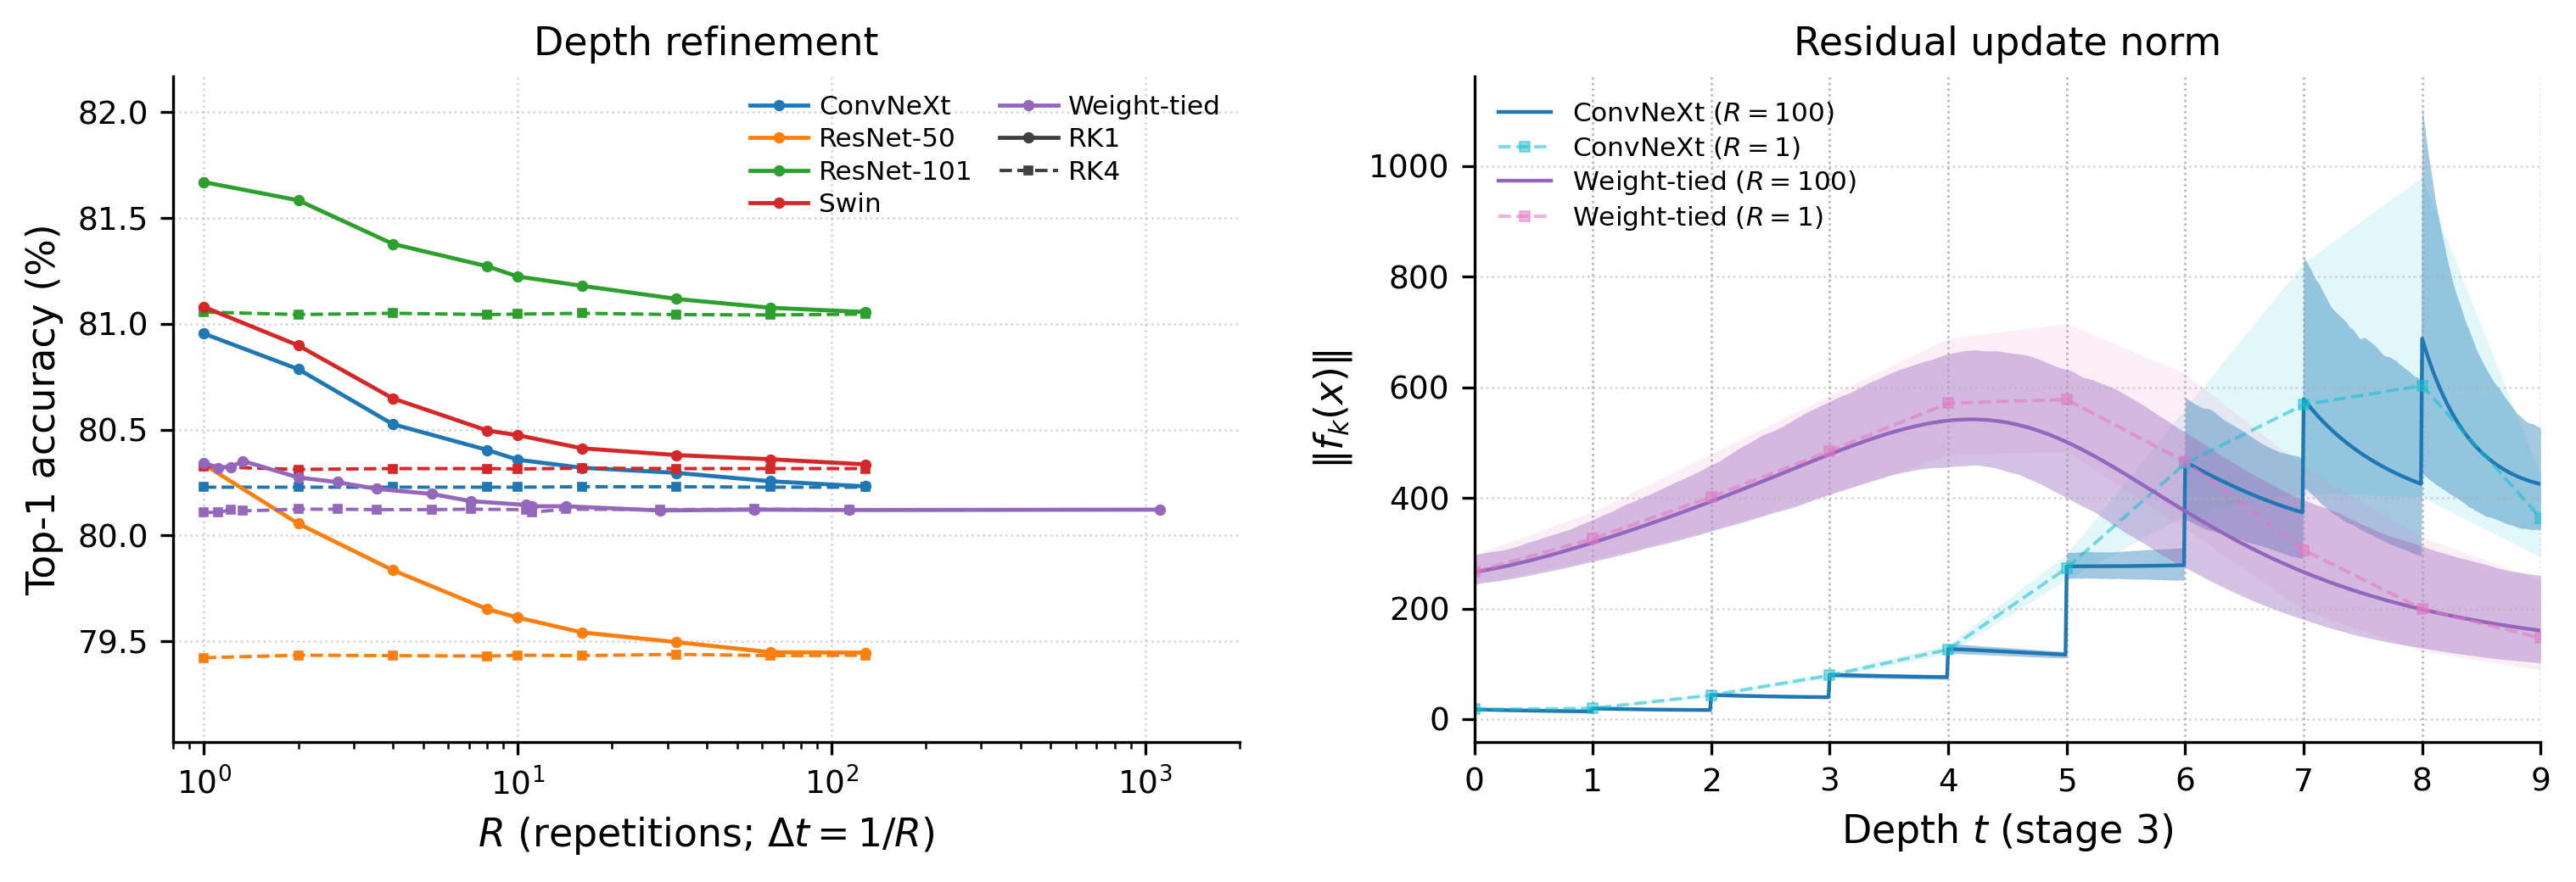
\includegraphics[width=\textwidth]{figures/teaser.png}
    \caption{\textbf{Left:} top-1 vs.\ repetitions $R$ (solid: Euler / RK1; dashed: RK4),
    with $\Delta t{=}1/R$ so $T{=}n$ is conserved
    (weight-tied: $nR$ applications of the shared block).
    \textbf{Right:} residual-field norm $\|f(x)\|$ along stage~3
    (mean and P5--P95 over 500 images). ConvNeXt is piecewise constant in depth;
    the weight-tied model is a single smooth autonomous field.
    See \cref{sec:teaser-b}.}
    \label{fig:teaser}
\end{figure*}

\Cref{sec:weight_tied} showed that one shared block nearly matches a standard
ConvNeXt stage~3 (independent per-block weights).
We now test whether residual blocks behave as one-step Euler updates of a vector field:
if so, repeating each update $R$ times with step $\Delta t{=}1/R$---without
fine-tuning---should preserve the trained horizon $T{=}n$ and the function the network
computes.
Convergence of the refinement by itself is not diagnostic, since any residual block
with Lipschitz $f$ has a continuous limit (\cref{app:random-init}); the informative
quantities are what the limit retains and how far the native path is from it.
We apply this probe to weight-tied and standard networks; the geometry of the
resulting trajectories is deferred to \cref{sec:geometrical_analysis}.

A residual block computes $x + f(x)$~\citep{he2016resnet}.
With step size $1$, that is exactly one step of the explicit Euler method for the ODE
$\dot x = f(x,t)$~\citep{e2017proposal,haber2017stable,lu2018beyond}.
Write the residual of block $i$ as
\begin{equation}
    f_i(x) \;=\; \mathrm{block}_i(x) - x.
    \label{eq:residual}
\end{equation}
Then the native network is one Euler step of size $1$ per block. Over a stage of $n$ blocks
(e.g.\ $n{=}9$ in ConvNeXt-T stage~3), starting from the output $x_0$ of the previous stage,
\begin{equation}
    x_{i+1} \;=\; x_i + f_i(x_i),
    \qquad
    x_n \;=\; x_0 + \sum_{i=0}^{n-1} f_i(x_i).
    \label{eq:euler-stage}
\end{equation}

Some argue that this algebraic form is already enough to call the network an Euler
solver~\citep{e2017proposal,haber2017stable,lu2018beyond},
but algebraic form alone is not sufficient evidence:
\citet{queiruga2020continuousindepthneuralnetworks} argue that ResNets fail to be meaningful
dynamical integrators beyond that syntactic similarity, and
\citet{sander2022residualneuralnetworksdiscretize} show that a ResNet approaches its associated
Neural ODE only when the residual maps vary smoothly in depth
(otherwise the discrete stack need not be a consistent discretization of a single continuous flow).

We suggest reading the stage as a \emph{sum of several ODEs}, one per block, where the network
is trained to solve each unit interval with a single Euler step.
The continuous object behind~\eqref{eq:euler-stage} is therefore
\begin{equation}
    x_n \;=\; x_0 + \sum_{i=0}^{n-1} \int_{i}^{i+1} f_i\bigl(x(t)\bigr)\,dt,
    \label{eq:sum-of-integrals}
\end{equation}
or, block by block,
\begin{equation}
    x_{i+1} \;=\; x_i + \int_{i}^{i+1} f_i\bigl(x(t)\bigr)\,dt.
    \label{eq:block-integral}
\end{equation}
Here the sum is the stack of residual blocks, and each integral is the continuous counterpart of
the one-step update in~\eqref{eq:euler-stage}: instead of taking one Euler step of size $1$,
we integrate $f_i$ over the unit interval $[i,i+1]$, keeping the horizon of each block equal to $1$.
For a stage with $n$ blocks trained at unit step, the stage horizon is therefore
\begin{equation}
    T \;=\; n
    \qquad\text{(ConvNeXt-T stage~3: $n{=}9$, so $T{=}9$).}
    \label{eq:horizon-T}
\end{equation}

\paragraph{Repetitions $R$.}
Throughout the paper we use a single refinement parameter $R$ (\emph{repetitions}).
For a non-tied stage, $R{=}2$ means each of the $n$ blocks is applied twice, for $nR$ residual
updates in total.
For a weight-tied stage, $R{=}2$ means the \emph{same} shared block is applied $nR{=}18$ times.
In both cases we set the Euler step from the trained horizon,
\begin{equation}
    \Delta t \;=\; \frac{1}{R}
    \qquad\Rightarrow\qquad
    T \;=\; nR\cdot\Delta t \;=\; n,
    \label{eq:delta-from-R}
\end{equation}
so refining never changes the integration time---only the resolution.

\textbf{Plain} interpolation keeps the field piecewise constant on each block and discretizes
the integral with $R$ Euler sub-steps of size $\Delta t = 1/R$:
\begin{equation}
    \int_{i}^{i+1} f_i\bigl(x(t)\bigr)\,dt
    \;\approx\;
    \sum_{r=0}^{R-1} \Delta t\, f_i\bigl(x_{i + r\Delta t}\bigr).
    \label{eq:plain-euler}
\end{equation}
Equivalently, over the whole stage the refined trajectory is
\begin{equation}
    x_T \;=\; x_0 + \sum_{i=0}^{T-1} \sum_{r=0}^{R-1} \Delta t\, f_i\bigl(x_{i + r\Delta t}\bigr),
    \qquad \Delta t = \tfrac{1}{R}.
    \label{eq:refined-stage}
\end{equation}
When $R{=}1$,~\eqref{eq:refined-stage} recovers the original network~\eqref{eq:euler-stage}.
As $R$ grows with $T{=}n$ fixed, the scheme approaches the continuous
limit~\eqref{eq:sum-of-integrals}; we also compare against Midpoint (RK2) and RK4 on the same horizon.

In a weight-tied stage the residual field is the same at every depth,
$f_i \equiv f$ for all $i$. Then~\eqref{eq:sum-of-integrals} collapses to a single
autonomous integral over $[0,T]$ with $T{=}n$:
\begin{equation}
    x_T \;=\; x_0 + \int_{0}^{T} f\bigl(x(t)\bigr)\,dt.
    \label{eq:weight-tied-ode}
\end{equation}
Inference uses $nR$ applications of $f$ with $\Delta t{=}1/R$; training uses $R{=}1$
($n$ steps of size $1$), hence $T{=}9$ for our shared ConvNeXt-T.


\subsubsection{Ablations}
\label{sec:looping-ablations}

We apply the refinement~\eqref{eq:refined-stage} (plain interpolation, $T$ conserved via
$\Delta t{=}1/R$) to our ConvNeXt-T, our weight-tied ConvNeXt-T, Swin-T, ResNet-50 and
ResNet-101 (ImageNet-1k validation, top-1).
\Cref{fig:teaser} (left) summarises the sweep over $R$; numbers are in
\cref{tab:r-ablation}.

Accuracy decreases monotonically as $R$ grows and plateaus at a continuous limit that
matches RK4.
Euler (RK1), Midpoint (RK2) and RK4 all converge to the \emph{same} accuracy once the
step is fine enough; full Mid/RK4 tables are in \cref{app:solvers}.
(Matched top-1 alone does not prove a shared state $x_T$; we check endpoint agreement
of the solvers later in \cref{app:solver-endpoints}.)
The trained network itself (Euler, $R{=}1$) is \emph{not} at that limit; it is the best
point of every sweep.
Keeping the nine steps of size $\Delta t{=}1$ but swapping Euler for RK4 already lands on
the limit, both in accuracy and in the stage-3 state (\cref{app:solver-endpoints}), and
costs $0.6$--$0.9$ points on the untied models ($0.2$ on the weight-tied one):
the decoder is tuned to the state produced by a single Euler step of size~$1$, not to
the flow it approximates.

\begin{table}[t]
    \centering
    \caption{Plain Euler refinement with $\Delta t{=}1/R$ ($T$ conserved). Top-1 (\%).
    For weight-tied, $R$ means $9R$ applications of the shared block
    (exact $9R$ when available; else nearest measured depth$^\ast$).
    ODE limit: RK4 at the finest step in each sweep.}
    \label{tab:r-ablation}
    \small
    \setlength{\tabcolsep}{2.8pt}
    \begin{tabular}{lrrrrr}
        \toprule
        $R$ ($\Delta t$) & CNX-T & Swin-T & R-50 & R-101 & Tied \\
        \midrule
        $1$ ($1$)       & 80.95 & 81.08 & 80.34 & 81.67 & 80.34 \\
        $2$ ($0.5$)     & 80.79 & 80.90 & 80.06 & 81.58 & 80.27 \\
        $4$ ($0.25$)    & 80.53 & 80.65 & 79.84 & 81.38 & 80.22$^\ast$ \\
        $10$ ($0.1$)    & 80.36 & 80.47 & 79.61 & 81.22 & 80.14$^\ast$ \\
        $32$ ($0.03$)   & 80.30 & 80.38 & 79.50 & 81.12 & 80.14$^\ast$ \\
        $128$ ($0.008$) & 80.23 & 80.34 & 79.45 & 81.06 & 80.12$^\ast$ \\
        \midrule
        ODE limit       & 80.23 & 80.32 & 79.43 & 81.05 & 80.12 \\
        Gap ($R{=}1\!\to$ODE) & $-0.72$ & $-0.76$ & $-0.91$ & $-0.62$ & $-0.22$ \\
        \bottomrule
    \end{tabular}
    \vspace{2pt}
    {\footnotesize $^\ast$Nearest measured shared depth at $T{=}9$:
    32, 96, 128, 1024 steps respectively (exact $9R$ would be 36, 90, 288, 1152).}
\end{table}

\paragraph{Wrong step size.}
Repeating blocks without shrinking the step (e.g.\ $R{=}10$ with $\Delta t{=}1$, so
$T$ grows tenfold) collapses every pretrained model to chance
($\approx 0.1\%$--$1\%$ top-1).
The same holds for the weight-tied network when $T$ leaves the trained horizon
(\cref{fig:horizon,fig:shared-fractional}).
The Euler step must be $\Delta t{=}1/R$, equivalently $T{=}n$ for an $n$-block stage
($T{=}9$ when $n{=}9$).
The trajectory dynamics behind this collapse are analysed in \cref{sec:beyond_horizon}.

\paragraph{Weight-tied fractional $R<1$.}
\Cref{fig:shared-fractional} reports the shared network at fixed $T{=}9$ with fewer
than nine steps ($R<1$, i.e.\ $9R$ applications with $\Delta t{=}1/R>1$); the numbers,
including Midpoint, are in \cref{tab:app-shared-t9}.
Large steps need a higher-order solver: at $R{=}4/9$ (4 steps), RK4 reaches $78.9\%$ while
Euler falls to $67.8\%$; Euler with $R{=}2/9$ ($\Delta t{=}4.5$) is unstable ($5.9\%$).
For $R\geq 7/9$, all three solvers sit within $0.3$ points of the trained baseline.

\begin{figure}[t]
    \centering
    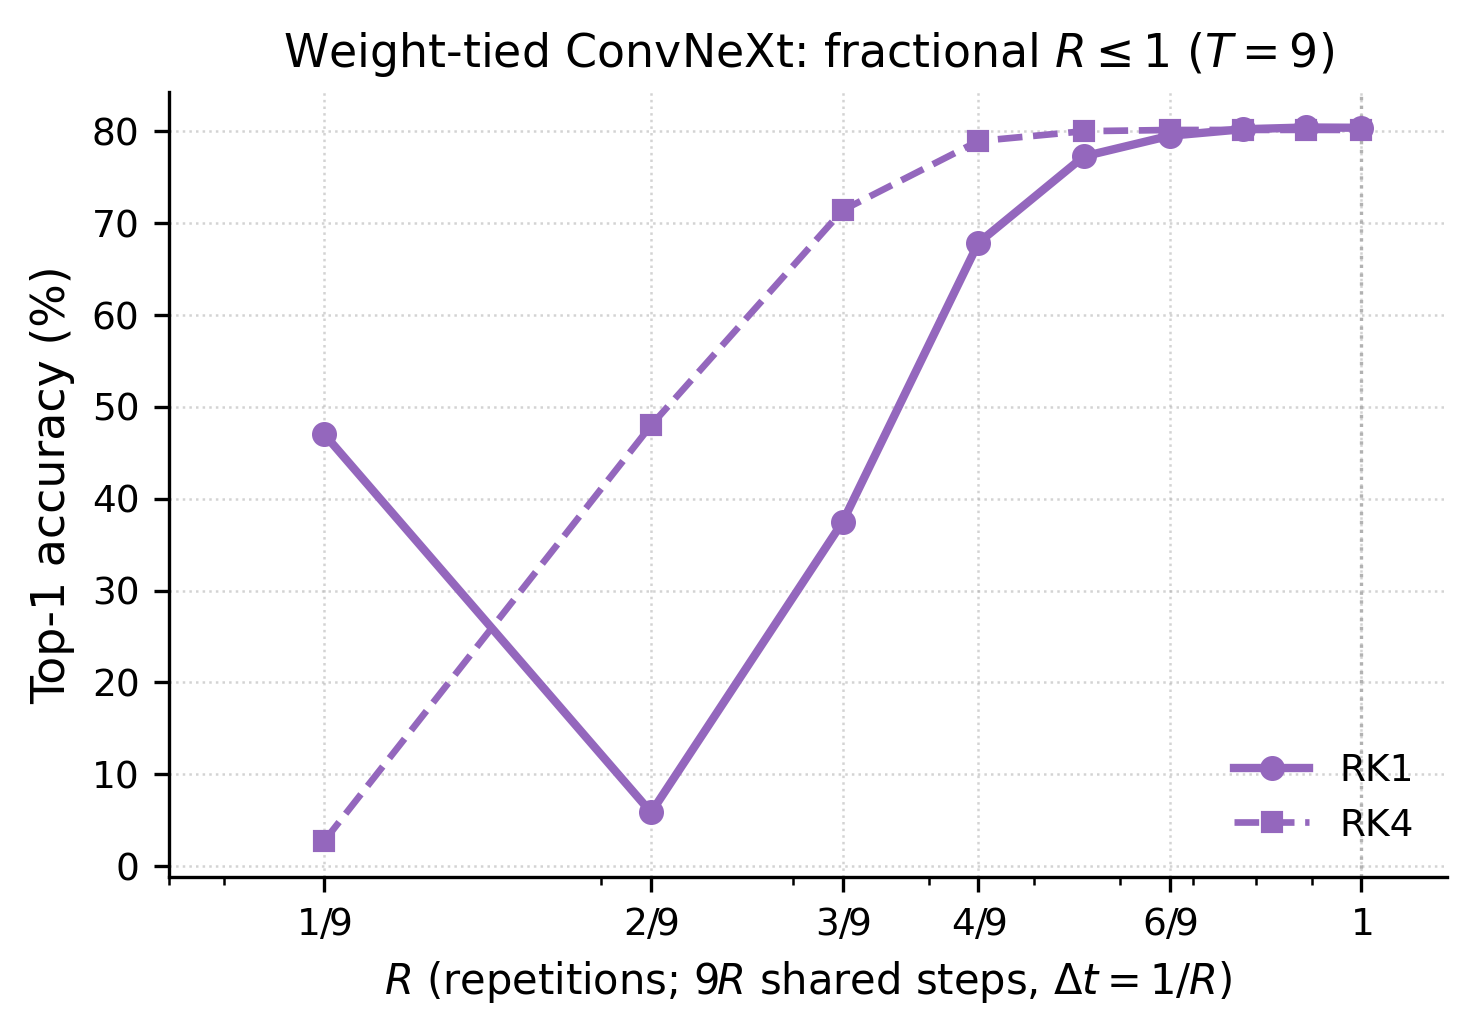
\includegraphics[width=\linewidth]{figures/shared_fractional.png}
    \caption{Shared ConvNeXt-T at fixed $T{=}9$ for fractional $R\leq 1$
    (RK1 solid, RK4 dashed).}
    \label{fig:shared-fractional}
\end{figure}

\paragraph{Horizon, not resolution.}
Varying the number of unit steps at $\Delta t{=}1$ (so $T$ grows) or varying $\Delta t$ at
fixed $R{=}1$ (9 steps; $T{=}9\cdot\Delta t$) both peak at $T{=}9$
(\cref{fig:horizon}): the classification head expects the state reached after that
integration time.
Integrating too short or too long degrades smoothly near $T{=}9$ and collapses far from it.
We conclude that the best Euler step is the one that preserves the trained horizon:
$\Delta t{=}1/R$ for every model (non-tied and weight-tied).

\begin{figure}[t]
    \centering
    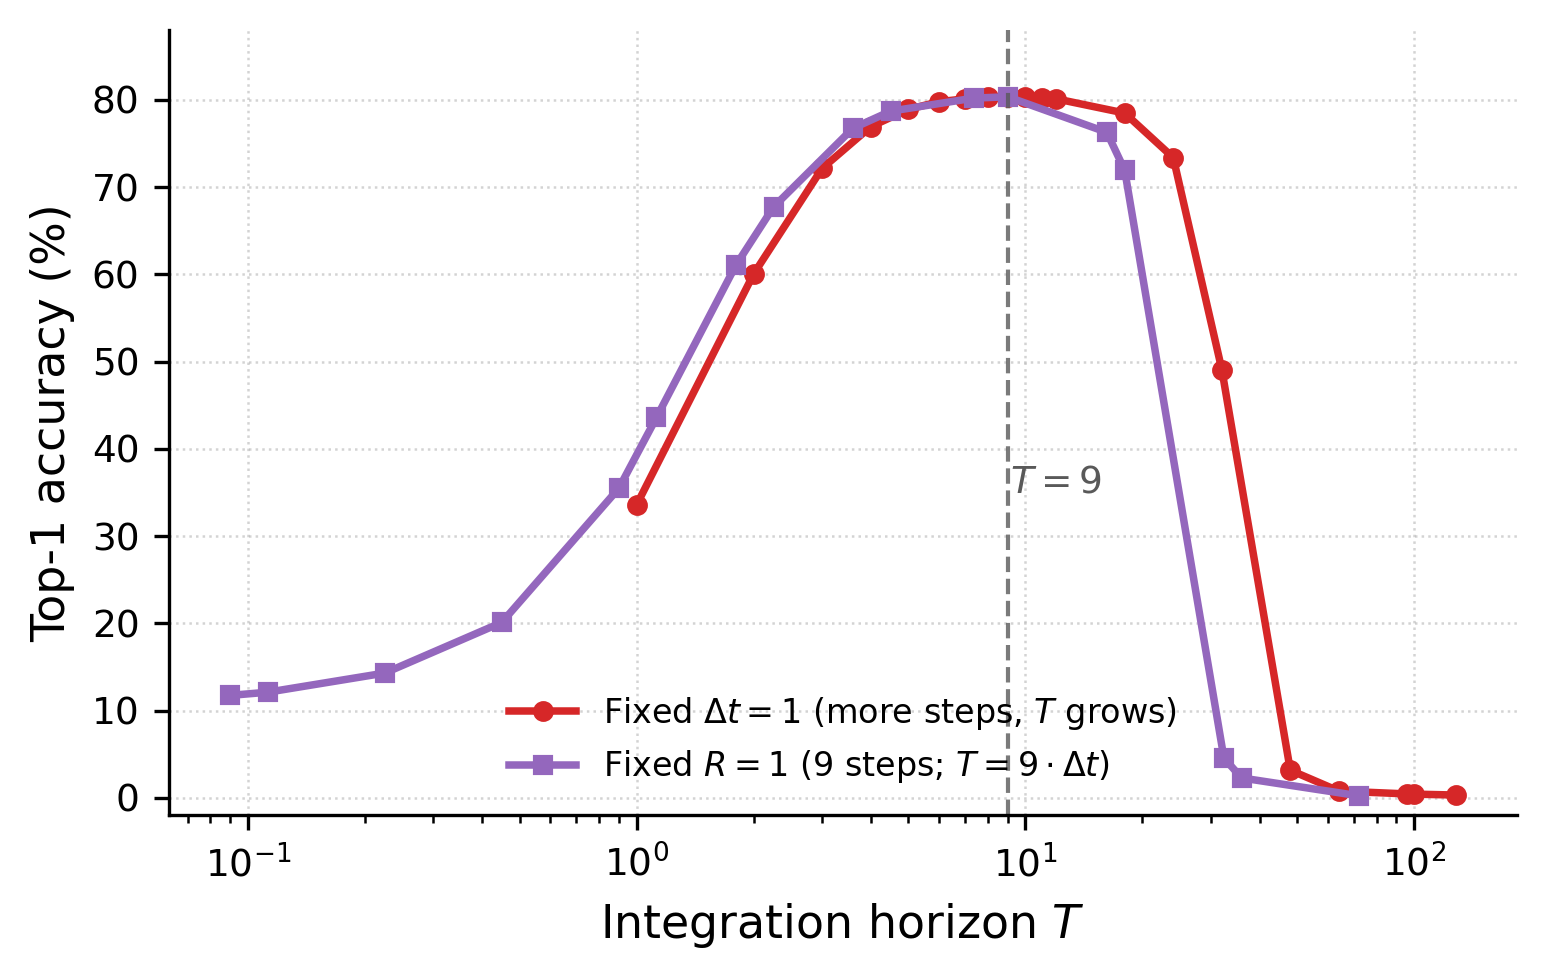
\includegraphics[width=\linewidth]{figures/horizon_ablation.png}
    \caption{Shared ConvNeXt-T: top-1 vs.\ horizon $T$.
    Red: fixed $\Delta t{=}1$, more steps ($T$ grows).
    Purple: fixed $R{=}1$ (9 steps), varying $\Delta t$ ($T{=}9\cdot\Delta t$).
    Both peak at the trained horizon $T{=}9$.}
    \label{fig:horizon}
\end{figure}

\paragraph{Do refined blocks land on the same $x$?}
Near-baseline accuracy does \emph{not} mean that $R$ Euler steps of size $1/R$
reproduce the unit-step state.
\Cref{fig:dist-r1} compares the refined ConvNeXt-T trajectory ($R{=}100$,
$\Delta t{=}0.01$) with the native $R{=}1$ trajectory on the same images, in $\ell_2$
distance (top, next to both state norms) and cosine similarity (bottom)
(massive channel removed from the metrics, see \cref{sec:massive_activations};
$N{=}500$ images).
Three facts stand out.
\begin{itemize}
    \item \textbf{Within each block} the refined trajectory moves \emph{toward} the
    parallel $R{=}1$ checkpoint: the distance decays and the cosine rises until the
    block ends, so the refinement is not drifting away from the one-step endpoint of
    that block.
    \item \textbf{Across blocks} the gap grows: the block-end distance rises from
    $\approx 5.6$ to $\approx 76$ at $t{=}9$, against $\|x\|\approx 203$ at the stage exit,
    i.e.\ a relative gap $\|x^{(R)}-x_{R{=}1}\|/\|x\|\approx 0.36$.
    \item \textbf{The gap is a rotation.} The block-end cosine drops from $0.99$ to $0.93$
    ($\sim\!21^\circ$), while $\|x\|$ differs by only $\approx 3\%$ ($203$ vs.\ $210$);
    a pure rescaling of that size would account for a distance of $\approx 7$, not $76$.
\end{itemize}
Each block therefore implements a \emph{different} map than its one-step counterpart
once the input has already drifted; local refinement stays contractive toward the
current block's $R{=}1$ target, but errors accumulate through the switched stack and
the final $x_T$ points in a different direction from the native one.

\begin{figure}[t]
    \centering
    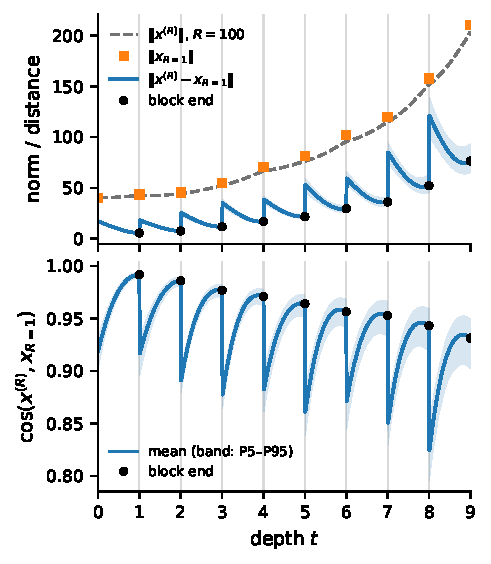
\includegraphics[width=\linewidth]{figures/dist_cos_r1.pdf}
    \caption{ConvNeXt-T, $R{=}100$, $\Delta t{=}0.01$, against the native $R{=}1$ path.
    \textbf{Top:} $\|x^{(R)}(t)-x_{R{=}1}\|$ (solid), with the state norms of both paths
    for scale (dashed: $R{=}100$; squares: $R{=}1$).
    \textbf{Bottom:} $\cos(x^{(R)},x_{R{=}1})$.
    Mean and P5--P95 over 500 images; massive channel ignored; dots mark block ends.
    The norms nearly coincide while the block-end gap grows with depth: the mismatch is
    mostly in angle.}
    \label{fig:dist-r1}
\end{figure}

\paragraph{Finetuning stage~4 and the head after unrolling.}
As a complementary check, we freeze stem and stages~1--3 and finetune only stage~4
and the classification head on the unrolled transport (horizon $T{=}9$ conserved).
On ConvNeXt-T with $R{=}3$ ($\Delta t{=}1/3$) this recovers $80.93\%$ top-1---within
$0.04$ points of the untied baseline ($80.97\%$).\footnote{Script:
\texttt{scripts/finetune\_s4\_r\_convnext.py}.
For contrast, $R{=}3$ with $\Delta t{=}1$ (broken horizon $T{=}27$) collapses to
$41\%$ \emph{without} finetuning (\texttt{convnext\_r3\_quick}).}
% TODO: sync Leonardo run directories for the numbers below.
The same protocol at the fine step used in \cref{fig:dist-r1} yields
$\mathrm{XX}\%$ top-1 for ConvNeXt-T at $R{=}100$ ($\Delta t{=}0.01$)
and $\mathrm{XX}\%$ for the weight-tied model at $R{=}100$ ($900$ shared steps, $\Delta t{=}0.01$)
after $10$ epochs at learning rate $10^{-6}$
(\texttt{finetune\_s4\_r100\_convnext.sh}, \texttt{finetune\_s4\_d900\_shared\_convnext.sh}).
So even though the refined stage-3 endpoint differs substantially from the native
$x_T$ in representation space, a light adaptation of the decoder largely restores
accuracy when $T$ is kept: the transport changes; the head can re-read it.

\paragraph{Takeaway.}
Three facts summarise the looping probe.
\emph{(i)~Discretisation.}
Refining the Euler step at fixed~$T$ does \emph{not} reproduce the native one-step
state: at $R{=}100$, after removing the massive channel, the stage-3 endpoint has
relative $\ell_2$ gap $\approx 0.36$ to the parallel $R{=}1$ path
(\cref{fig:dist-r1}) and cosine $\approx 0.93$ ($\sim\!21^\circ$), so the mismatch is
mostly angular rather than a pure rescaling of $\|x\|$.
The weight-tied stage does not accumulate this error: its cosine to the $R{=}1$ path
settles at $\approx 0.98$ (relative gap $\approx 0.20$) instead of falling block after
block (\cref{sec:refinement_error}).
\emph{(ii)~Continuous limit.}
That gap is \emph{not} solver noise: Euler and RK4 at the same fine step, and Euler
$R{=}100$ vs.\ $R{=}200$, agree on $x_T$ to relative distance $\ll 10^{-2}$
(\cref{app:solver-endpoints}).
A continuous limit of the piecewise residual field therefore exists, but it is not
the trained $R{=}1$ discretisation.
Neither fact is specific to training.
A random-initialisation control (\cref{app:random-init}) shows that the blocks of all
five architectures, random or trained, converge to a single $\hat x_T$ under refinement.
How far the one-step path lies from that limit is governed mainly by how far each block
moves the state, $\|f_i(x_i)\|/\|x_i\|$: weights trained to be used once produce steps of
$30$--$90\%$ of $\|x\|$ and sit $10$--$21^\circ$ from their limit, too far for one Euler step
to track the flow.
At the same relative step, training moves that distance in an architecture-dependent
direction: trained Swin-T and ConvNeXt-T are closer to their limit than a random field
($19.5^\circ$ vs.\ $47.6^\circ$, $21.1^\circ$ vs.\ $30.2^\circ$), the weight-tied model is level
with it ($10.9^\circ$ vs.\ $11.9^\circ$), and the ResNets are farther.
What distinguishes the trained networks is therefore not \emph{whether} the refinement
converges but \emph{how} the trajectory is built: one shared block applied throughout
the stage versus nine different blocks applied once each.
\Cref{sec:geometrical_analysis} contrasts the two regimes.
\emph{(iii)~Accuracy.}
Top-1 nevertheless barely moves under refinement without training, because the head
cares about class margins, not isometry of the full feature space.
Finetuning stage~4 and the head recovers $80.93\%$ at $R{=}3$ and
$\mathrm{XX}\%$ / $\mathrm{XX}\%$ for ConvNeXt-T / weight-tied at $R{=}100$
% TODO: fill XX from Leonardo S4+head runs (10 epochs, lr=1e-6).
---essentially the baseline once the decoder adapts.
In short: residual blocks admit a well-defined fine-step flow, as any Lipschitz residual
field does; their single unit step is too large to be a consistent solver of that flow;
the flow nonetheless retains the network's function (the limit keeps $\approx 80\%$ top-1,
which a random field cannot show), accuracy survives because the head is tolerant, and a
light S4+head adaptation closes almost all of the remaining gap.

Influenced by continuous-in-depth models~\citep{queiruga2020continuousindepthneuralnetworks,chang2018multilevel},
we also tried replacing the piecewise-constant schedule
$\theta_t=\theta_{\lfloor t\rfloor}$ by a bilinear blend of consecutive block weights.
It performs relatively badly on every architecture (e.g.\ $-6.6$ points on ConvNeXt-T at
$R{=}128$ vs.\ plain); full numbers and the residual-norm trajectories are in
\cref{app:bilinear}.

\subsubsection{Piecewise vs.\ smooth residual fields}
\label{sec:teaser-b}

\Cref{fig:teaser}~(right) makes the dynamical difference between the two regimes concrete.
In the non-tied ConvNeXt, $\|f_k(x)\|$ is approximately constant inside each block and
jumps at integer depths: a \emph{smooth function by parts}, i.e.\ an autonomous field on
each unit interval $[i,i+1]$ with discontinuous switches of $\theta$ between blocks
(\cref{eq:sum-of-integrals}).
In the weight-tied model the same shared $f$ is applied for the whole stage, so the
residual norm evolves as one continuous curve that rises and then decays
(\cref{eq:weight-tied-ode}).
Markers at $R{=}1$ sit on those curves; refining to $R{=}100$ fills in the
intra-block path without changing its global shape.
This is the geometric counterpart of the accuracy tables: refining a switched stack
converges to a slightly worse continuous limit, while refining a shared field stays near
the trained accuracy as long as $T$ is held fixed.
\Cref{sec:geometrical_analysis,sec:overparametrized_undoing} analyse these trajectories
in more detail---in particular, how untied blocks redirect the state between integer
depths even though each intra-block piece remains integrable.

\subsection{Geometrical analysis of feature trajectories}
\label{sec:geometrical_analysis}

In this section we analyze the geometry of the trajectories regarding the weight-tied convnext vs the standard convnext.
We also compare the standard convnext with resnet and swin, whose properties are very similar since they are non weight-tied and
the network learned to make the blocks perform an unique functionality of one step, so there is no reason for the network to learn a more
complex dynamic.

\subsubsection{Massive activations excluded from analysis}
\label{sec:massive_activations}

After analyzing some trajectories on our first aproach, they seemed too homogeneos in convnext and swin cases, so we analyzed the features and
founded the so called massive activations \cite{sun2024massiveactivationslargelanguage}. In convnext shared and non-shared there is one channel that grows indifinetly.
We did a similar analysis and concluded the same as \cite{sun2024massiveactivationslargelanguage}

\subsubsection{Trajectories of weight-tied convnxt vs standard convnext}


\subsubsection{Trajectory analysis of weight-tied convnext}
\label{sec:refinement_error}
Inpired by some of the metrics of \cite{pandey2026trajectorygeometrytransformerrepresentations} we perform an analysis of the trajectories
ignoring the massive channels of Convnext and the massive tokens of swin. Resnet does not show signs of massive activations.

In weight-tied convnext we can see in Figure \ref{fig:teaser} right the norm of the velocity, that is $f(x(t))$ that has a shape of a bell curve.
This information only shows if the point is moving or not, but it doesn't tell if it rotates or move towards the same direction.
That's why we plot several new metrics:

\textbf{Acceleration}

Here we decompose the acceleration vector into the sum of two components: The tangential and normal accelerations with respect to the velocity.
Note, that in a high-dimentional space of 300,000 dimensions (the case of Stage 3 in convnext), there are 299.999 dimentions that are normal with the velocity, and only 1 that is tangent.
The tangent component can be negative or positive with respect to the velocity that is, it reduces or increases the current velocity in this 1D line, but we cna only analyze the norm of the normal acceleration.
Even in a such space, that tangential acceleration has a big representation.

We can see

\textbf{Angular acceleration}
\textbf{Trajectory curvature}

\textbf{The shape of the trajectory}

With all this tools, we conclude that the trajectory at the start rotates at high speeds, giving the trajectory a high curvature,
but with low velocity norm, that implies that it does small steps changing constantly of direction. The model is computing the direction where it has to accelerate the point to.

After that, the model starts to accelerate towards one direction, angular speed decreases, norm of angular acceleration increases due to the reduction of velocity
the result is a major reduction on the curvature of the trajectory, while tangential acceleration hits its maximum. The model is expanding the most important features.

Finally, angular acceleration decreases, tangential acceleration rapidly decreases, becoming negative, the velocity decreases, the angular velocity increases again, and curvature raises again. We have the same
scenario as in the first phase. The model is refining features again.

We observe that for the 500 images we analyzed, the trajectory is mostly of this form. But in the variance analysis,
the velocity has its maximum variance on the second phase since the model is pushing the features of different classes apart from the origin in different directions.

\subsubsection{Refinement error: accumulated vs.\ bounded}
\label{sec:refinement_error}

\begin{figure*}[t]
    \centering
    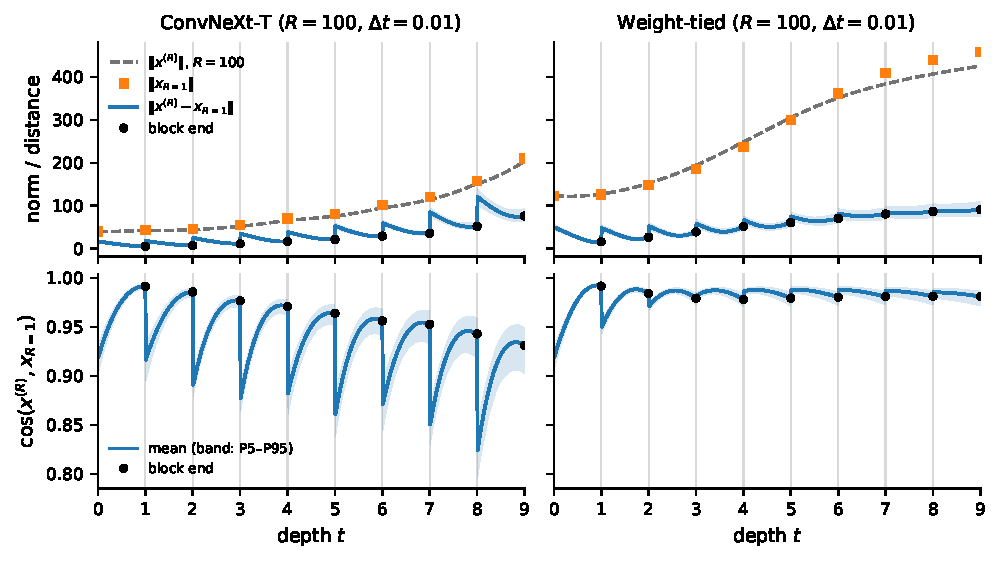
\includegraphics[width=\textwidth]{figures/dist_cos_r1_compare.pdf}
    \caption{Refined vs.\ native ($R{=}1$) stage-3 path for the standard (left) and
    weight-tied (right) ConvNeXt-T.
    \textbf{Top:} $\|x^{(R)}-x_{R{=}1}\|$ (solid) with both state norms for scale
    (dashed: refined; squares: native).
    \textbf{Bottom:} $\cos(x^{(R)},x_{R{=}1})$.
    Mean and P5--P95 over the same 500 images; massive channel ignored; dots mark the end
    of each native step.
    The switched stack accumulates angle at every block; the shared field saturates.}
    \label{fig:dist-r1-compare}
\end{figure*}

\Cref{fig:dist-r1-compare} repeats the comparison of \cref{fig:dist-r1} for the
weight-tied network.
Both models start the same way: after the first native step the cosine to the $R{=}1$
path is $0.99$.
They then diverge.
In the standard ConvNeXt-T the block-end cosine keeps falling, to $0.93$ at $t{=}9$:
each block receives an input that has already drifted and adds its own discretisation
error on top.
In the weight-tied model it settles at $\approx 0.98$ after two or three steps and stays
there for the rest of the stage, so a single autonomous field keeps the refinement error
bounded instead of accumulating it.
The norms also behave differently: in ConvNeXt-T they nearly coincide ($203$ vs.\ $210$),
whereas the weight-tied refined path ends about $7\%$ shorter ($427$ vs.\ $458$), so part
of its smaller gap is radial.
% TODO: relate the bounded error to the contractivity of the shared field.

\subsubsection{Integrating beyond the trained horizon}
\label{sec:beyond_horizon}
% TODO: constant velocity regime: f(x) saturates, x grows along a fixed direction for T >> n.
There is big difference between weight-tied convnext and standard convnext: First one reaches a velocity plateau
where the input just grows indifinetly in the same direction.

In standard convnext, swin and resnet are different, we used R=100 with euler step 1,
since the blocks use different parameters and the network was not trained to reuse params,
it has a similar dynamics as the R=100 with Euler step of 0.01 but with more magnitude.

\subsection{Are over-parametrized networks undoing what the previous layers have done?}
\label{sec:overparametrized_undoing}

\Cref{sec:weight_tied} showed that one shared stage-3 block nearly matches nine
independent ones ($-0.61$ top-1 points, $33\%$ fewer parameters).
A natural explanation is that the untied stack is over-parametrised along depth:
consecutive blocks need not push the state in a coherent direction, and part of
what block $k{+}1$ does can cancel what block $k$ just did.
We test that claim directly on feature trajectories, using the same 500 ImageNet
validation images (one per class) as in \cref{sec:geometrical_analysis}, stage~3
only, with the massive channel removed (\cref{sec:massive_activations}).

\paragraph{Setup.}
For each image we integrate the stage from $t{=}0$ to $t{=}9$ at native resolution
($R{=}1$) and under Euler refinement ($R{=}100$, $\Delta t{=}0.01$), and reduce every
spatial feature coordinate whose net displacement $|\Delta_i|=|x_i(9)-x_i(0)|$ is above
the per-image median.
We partition the trajectory into the nine unit intervals $[k,k{+}1]$ (native blocks
in ConvNeXt-T; the same time bins in the weight-tied model) and write
$\mathrm{d}x_k$ for the displacement of a coordinate over interval $k$.
The scalars we report are means $\pm$ std over the 500 images
(\cref{tab:undo}):
\begin{itemize}
    \item \emph{straightness}: $\|\sum_k\mathrm{d}x_k\|\,/\,\sum_k\|\mathrm{d}x_k\|$
    in feature space (path length vs.\ net displacement);
    \item \emph{wasted motion}: $1-\sum_i|\mathrm{net}_i|/\sum_{k,i}|\mathrm{d}x_{k,i}|$,
    the fraction of per-coordinate travel that cancels before $t{=}9$;
    \item $\cos(\mathrm{d}x_k,\mathrm{d}x_{k+1})$: mean cosine between consecutive
    block displacements;
    \item \emph{undo fraction}: when $\mathrm{sign}(\mathrm{d}x_k)$ flips at the next
    block, the cancelled mass
    $\min(|\mathrm{d}x_k|,|\mathrm{d}x_{k+1}|)$ normalised by $\sum|\mathrm{d}x_k|$;
    \item \emph{zig-zag share}: mass-weighted share of coordinates that reverse at
    least twice across the nine blocks;
    \item \emph{sign flips at $t\in\mathbb{N}$}: fraction of consecutive steps whose
    sign changes exactly at integer depths (block boundaries).
\end{itemize}

\begin{table*}[t]
    \centering
    \caption{Pooled stage-3 trajectory statistics over 500 ImageNet images
    (massive channel ignored; coordinates with $|\Delta_i|$ above the per-image median).
    Weight-tied vs.\ standard ConvNeXt-T at native ($R{=}1$) and refined ($R{=}100$)
    resolution. Mean $\pm$ std across images.}
    \label{tab:undo}
    \scriptsize
    \setlength{\tabcolsep}{3.5pt}
    \resizebox{\textwidth}{!}{%
    \begin{tabular}{llccccccccc}
\toprule
Model & $R$ & straightness & wasted motion & monotone share & $\cos(\Delta x_k,\Delta x_{k+1})$ & reversal rate & undo fraction & zig-zag share & sign flips at $t\in\mathbb{N}$ & median $t_{50}$ \\
\midrule
Weight-tied ConvNeXt & 100 & 0.78$\pm$0.02 & 0.19$\pm$0.01 & 0.73$\pm$0.02 & 0.92$\pm$0.01 & 0.11$\pm$0.01 & 0.02$\pm$0.00 & 0.14$\pm$0.02 & 0.00$\pm$0.00 & 4.09$\pm$0.16 \\
ConvNeXt-T & 100 & 0.50$\pm$0.01 & 0.48$\pm$0.01 & 0.21$\pm$0.01 & 0.17$\pm$0.01 & 0.45$\pm$0.00 & 0.25$\pm$0.00 & 0.90$\pm$0.00 & 0.45$\pm$0.00 & 7.21$\pm$0.15 \\
Weight-tied ConvNeXt & 1 & 0.72$\pm$0.02 & 0.25$\pm$0.02 & 0.63$\pm$0.03 & 0.77$\pm$0.03 & 0.18$\pm$0.01 & 0.05$\pm$0.01 & 0.34$\pm$0.03 & 0.18$\pm$0.01 & 5.00$\pm$0.09 \\
ConvNeXt-T & 1 & 0.50$\pm$0.01 & 0.48$\pm$0.01 & 0.22$\pm$0.01 & 0.16$\pm$0.01 & 0.45$\pm$0.00 & 0.25$\pm$0.00 & 0.90$\pm$0.00 & 0.45$\pm$0.00 & 7.82$\pm$0.38 \\
\bottomrule
\end{tabular}

    }
\end{table*}

\begin{figure*}[t]
    \centering
    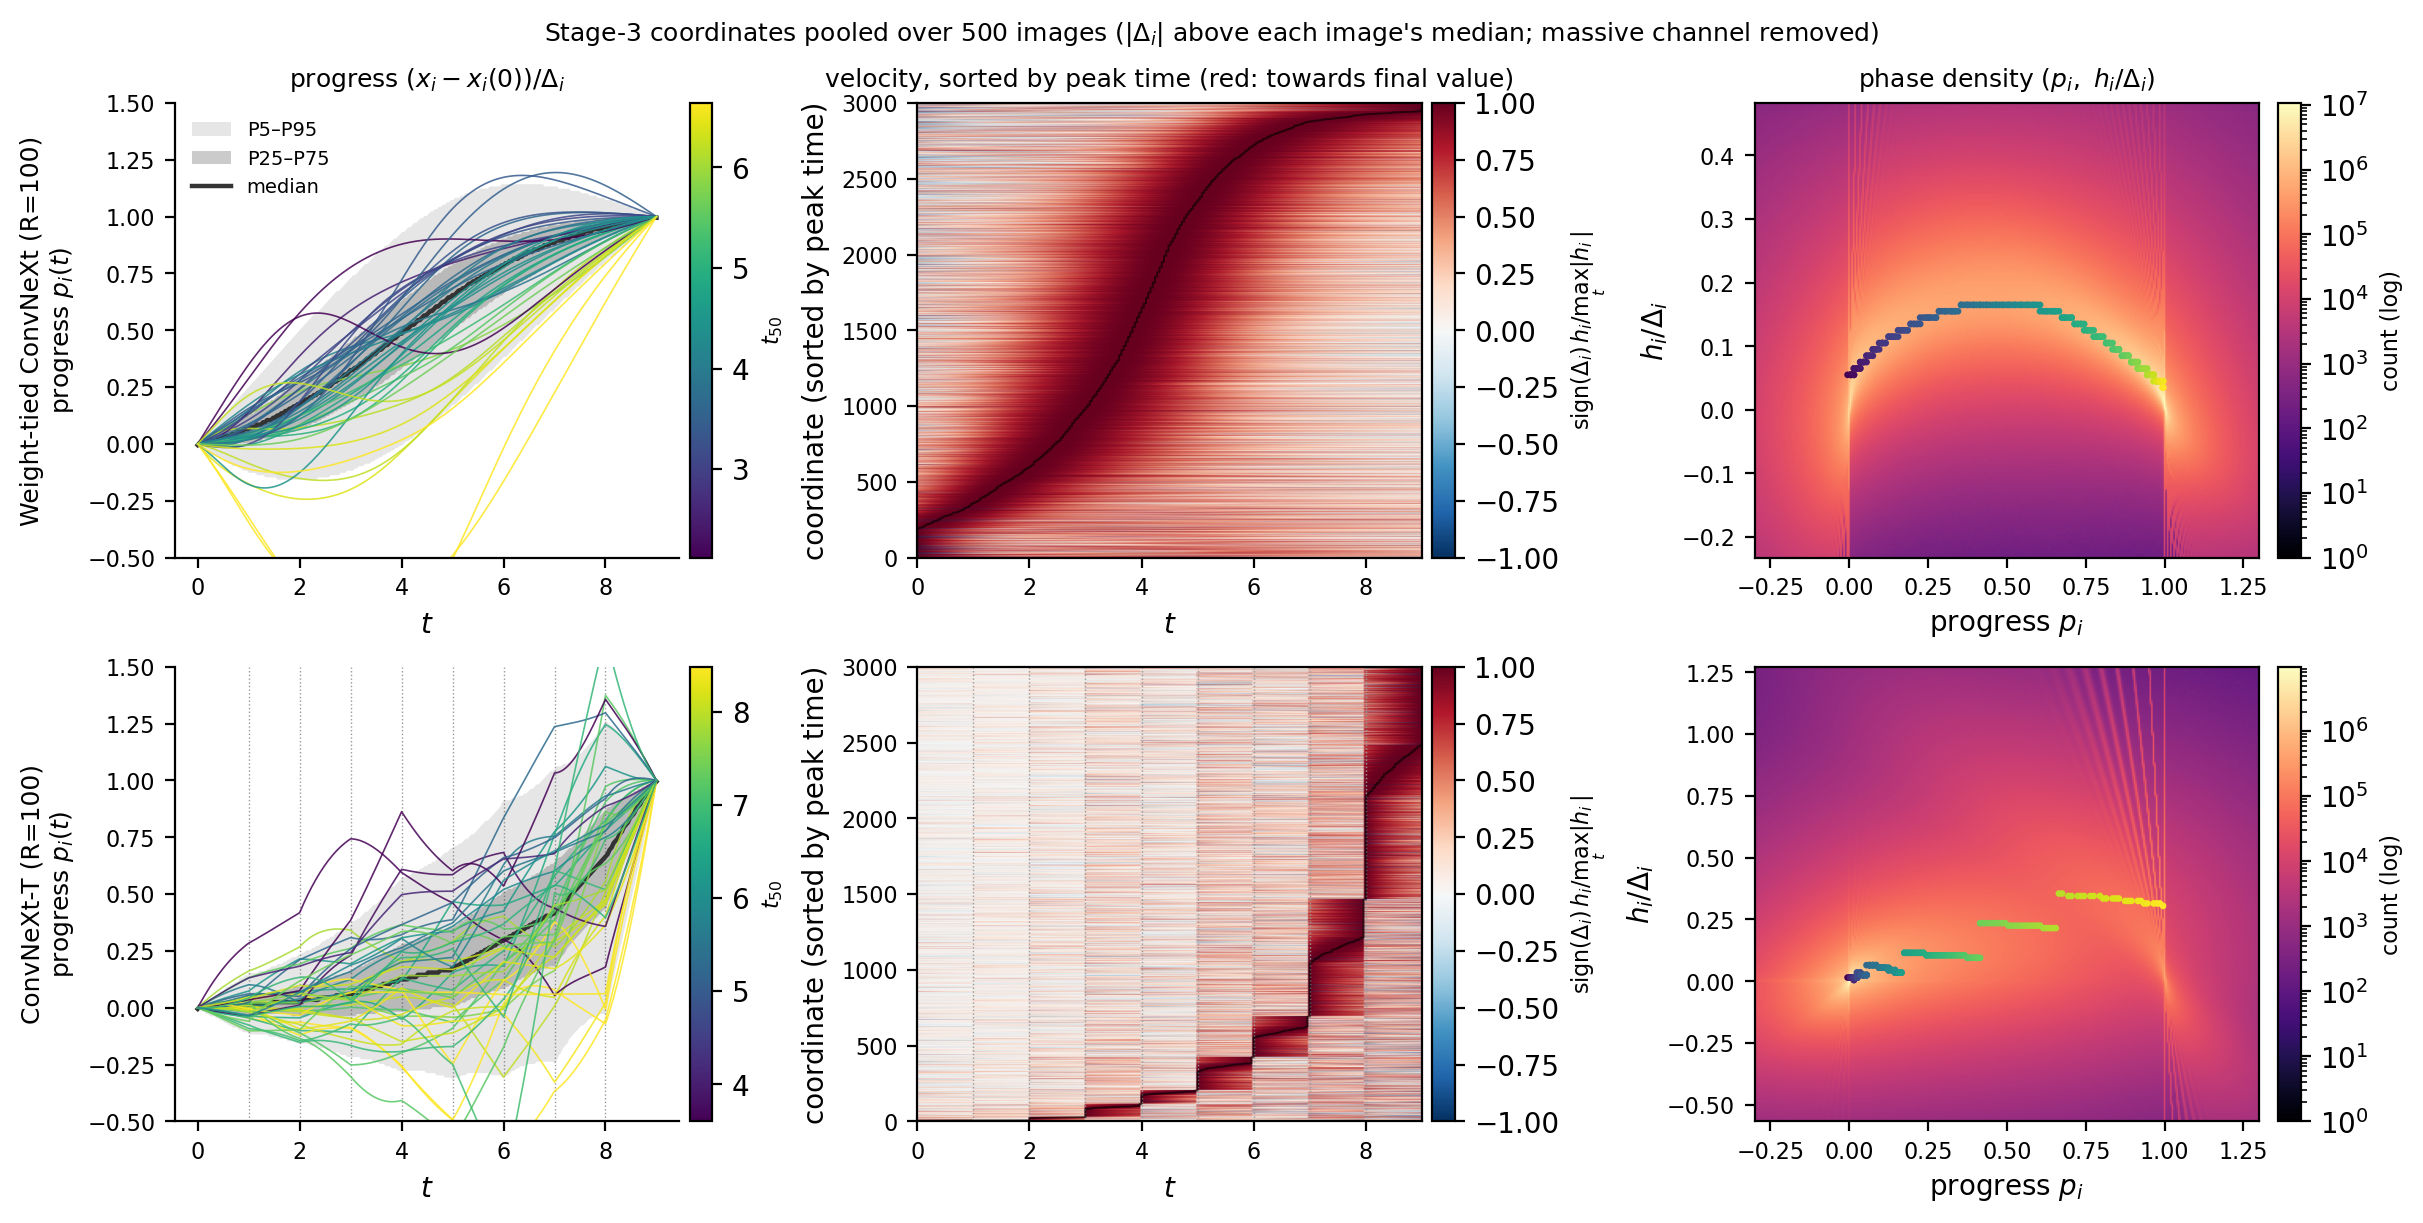
\includegraphics[width=\textwidth]{figures/pooled_dynamics.png}
    \caption{Stage-3 coordinates pooled over 500 images ($R{=}100$; massive channel
    removed; $|\Delta_i|$ above the per-image median).
    \textbf{Top:} weight-tied ConvNeXt; \textbf{bottom:} ConvNeXt-T.
    \textbf{Left:} progress $p_i(t)=(x_i(t)-x_i(0))/\Delta_i$ (median and P5--P95;
    thin lines: random coordinates).
    \textbf{Middle:} velocity toward the final value, coordinates sorted by peak time
    (red: toward the end state; blue: away).
    \textbf{Right:} phase density $(p_i,\,h_i/\Delta_i)$.
    The shared field advances mostly monotonically; the switched stack reverses and
    rewrites features between blocks.}
    \label{fig:pooled-dynamics}
\end{figure*}

\paragraph{Results.}
\Cref{tab:undo} and \cref{fig:pooled-dynamics} give a consistent picture.
Under refinement ($R{=}100$), the weight-tied model is nearly monotone along depth:
straightness $0.78$, wasted motion $0.19$, consecutive-block cosine $0.92$, undo
fraction $0.02$, and zig-zag share $0.14$.
Sign changes at integer times are essentially absent ($0.00$).
ConvNeXt-T, with nine independent blocks, sits at the opposite extreme: straightness
$0.50$, wasted motion $0.48$ (almost half of the travel cancels), cosine $0.17$,
undo fraction $0.25$ ($\approx 12\times$ the shared value), and zig-zag share $0.90$.
Nearly half of the sign flips ($0.45$) fall exactly on block boundaries---the
discontinuities of the switched field in \cref{sec:teaser-b}, not an artefact of a
coarse step.
Native resolution ($R{=}1$) barely changes the ConvNeXt-T numbers; refining only
makes the shared field look cleaner (undo $0.05\to 0.02$), which matches the bounded
refinement error of \cref{sec:refinement_error}.

\paragraph{Functional progress along depth.}
Geometry shows wasted motion; a complementary probe asks when the stage~3 state
becomes usable by the rest of the network.
For each $k{=}1,\ldots,9$ we stop after the $k$-th residual block and classify with
the model's own trained downsample, stage~4 and head---no remaining stage~3 blocks
(\cref{fig:prefix-acc}; full ImageNet validation).
Under weight tying the top-1 rises early and smoothly: $33.6\%$ after one block,
$72.2\%$ after three, and $78.9\%$ by block~5, already close to the final
$80.3\%$.
On standard ConvNeXt-T the same frozen decoder stays weak for longer
($11.5\%$, $33.2\%$, $66.9\%$ at those depths) and only approaches the final
$81.0\%$ in the last few blocks.
Mid-stage accuracy is not a claim that early features lack information---the head
was trained on $x_T$---but it does show that the tied path enters the decoder's
operating region steadily, whereas the untied path aligns with that region late,
consistent with a transport that rewrites features before committing.

\begin{figure}[t]
    \centering
    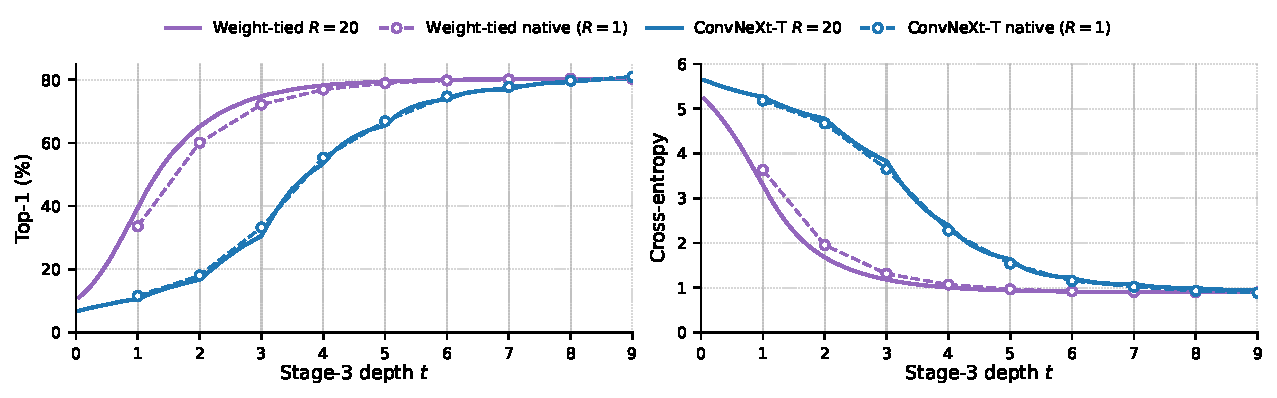
\includegraphics[width=0.7\linewidth]{figures/prefix_s4_head_acc.pdf}
    \caption{ImageNet top-1 of each model's trained stage~4+head on stage~3
    prefixes: after $k$ residual blocks, skip the rest of stage~3 and decode.
    Weight-tied features become usable earlier and more evenly; ConvNeXt-T
    concentrates most of the gain toward the end of the stage.}
    \label{fig:prefix-acc}
\end{figure}

\paragraph{Reading.}
Untied stage~3 does not implement nine steps of one transport: consecutive blocks
often point in weakly related or opposing directions and cancel a large fraction of
each other's work.
The weight-tied network cannot cancel itself in that way---a single autonomous field
has no ``next block'' with different weights---and the geometry shows almost no
undoing.
\Cref{fig:prefix-acc} makes the same contrast in function space: tied depth builds
decoder-ready features gradually, while untied depth postpones most of the usable
progress.
That is why sharing the nine blocks costs less than one top-1 point
(\cref{sec:weight_tied}): much of the untied capacity along depth is spent
rewriting features rather than accumulating a coherent displacement toward $x_T$.
The residual accuracy gap to the baseline is then more plausibly attributed to the
small, non-cancellable specialization that independent $\theta_k$ still provide, not to
a fundamentally different dynamical mechanism.

\subsection{Shared field with per-block deltas}
\label{sec:deltas}

% TODO: fine-tuning $\theta_i = \theta_{\mathrm{shared}} + \delta_i$ on top of the
% weight-tied stage-3 checkpoint; comparison to baseline and shared-only.


\section{Discussion}
\label{sec:discussion}

\Cref{tab:headline} collects the measurements that carry our reading.
The same residual algebra $x+f(x)$ supports two different transports, and refinement
at fixed horizon makes the difference visible without retraining either model.

\begin{table}[t]
    \centering
    \caption{Headline measurements on ImageNet-1k.
    Top-1 and ODE limit from \cref{tab:r-ablation}; straightness (Str.) and consecutive
    block cosine at $R{=}1$ (\cref{tab:coherence,app:arch-transport}); parameters from
    \cref{sec:weight_tied}.
    Swin-T and the ResNets are torchvision checkpoints that we did not retrain.}
    \label{tab:headline}
    \small
    \setlength{\tabcolsep}{2.6pt}
    \begin{tabular}{lrrrrrr}
        \toprule
        Model & Params & $R{=}1$ & ODE & Gap & Str. & $\cos_{k,k+1}$ \\
        \midrule
        ConvNeXt-T         & 28.59M & 80.96 & 80.23 & $-0.73$ & 0.50 & 0.16 \\
        Weight-tied S3     & 18.97M & 80.34 & 80.12 & $-0.22$ & 0.72 & 0.77 \\
        All-stages tied    & 8.68M  & 78.99 & --    & --      & --   & --   \\
        Swin-T             & --     & 81.08 & 80.32 & $-0.76$ & 0.80 & 0.43 \\
        ResNet-50          & --     & 80.34 & 79.43 & $-0.91$ & 0.37 & $-0.11$ \\
        ResNet-101         & --     & 81.67 & 81.05 & $-0.62$ & 0.16 & 0.01 \\
        \bottomrule
    \end{tabular}
\end{table}

\paragraph{A staircase path.}
The untied ConvNeXt-T stage does not move back and forth: every block's increment survives to the end of the stage ($s_k>0$ for every image and
block), and consecutive increments are positively correlated (cosine $0.17$) where
random blocks of matched strength are uncorrelated.
Each block writes mostly in a new direction, so the net displacement grows more like
the square root of the number of steps than like their sum.
Straightness places it halfway between random blocks and the shared field
($0.33$, $0.50$, $0.78$), and the detour is made at the block switches, where the
heading turns by $80^\circ$ and $45\%$ of the coordinates of the velocity change sign;
inside a block the path is a shallow arc whose length exceeds its chord by $1.5\%$.
These statistics are already present at native resolution (for the untied stage
$R{=}1$ and $R{=}100$ agree to within $0.01$ in straightness and cosine), so they describe the trained
network and not the refinement.

\paragraph{Why does one field nearly match nine?}
The shared stage reaches $80.34\%$ against $80.96\%$ with $33\%$ fewer parameters.
Our measurements are consistent with a simple reading: the shared field, which must act
sensibly on every state it visits, moves the state along a coherent direction and
reaches the decoder's operating region earlier (prefix top-1 $74.7\%$ at $t{=}3$
against $30.6\%$), while the nine untied blocks spread the same transport over nine
nearly orthogonal steps and make most of the final displacement in the last blocks.
They do not show that the untied directions are unnecessary, nor what the $0.62$ points
buy.
Nearly orthogonal increments could carry information that a single field cannot
write, and the accuracy gap itself comes from runs with different learning rates and
warmups (\cref{app:training}).
Why the coherent field nearly matches the staircase remains an open question.

\paragraph{Refinement as a probe.}
Every architecture converges to a continuous limit at fixed $T$ that keeps the function
within $0.22$ to $0.91$ points, although it sits $11^\circ$ to $21^\circ$ from the native
state (\cref{app:solver-endpoints}); breaking the horizon instead collapses every
network.
A trained stage is thus a sequence of one-step solves, each replaceable by a finer
integral of the same block, but not a Neural ODE with weights smooth in depth
(\cref{app:bilinear}).
The probe needs no retraining, the Gram statistics only need block increments and prefix
decoding only needs the trained downstream network, so all three apply to any residual
stream, including looped transformers~\citep{dehghani2019universal,giannou2023looped},
the weight-tied counterpart of our shared stage.

\paragraph{Limitations.}
All results are on ImageNet-1k classification, and the trained tied and untied stages
are one pair of ConvNeXt-T runs, without seeds and with different learning-rate
schedules.
The open question above is the main one: we describe how the two transports differ,
not why the difference costs only $0.62$ points.
The channel basis is not privileged, so per-coordinate readings of the trajectories
(sign changes between blocks) are partly determined by the Gram matrix and partly by the
basis (\cref{app:per-coordinate}); we base our claims on Gram statistics only.
The metrics exclude the massive ConvNeXt channel and the Swin corner tokens, and we
have not tested whether the ReLU after the ResNet sum explains its negatively correlated
increments (\cref{app:arch-transport}).

\paragraph{Toward more expressivity per parameter.}
The two regimes suggest a design space between them: a shared field with small
per-block corrections, or cycles of a few shared blocks, would interpolate between an
autonomous and a switched flow.
Related schemes exist for convolutional networks~\citep{savarese2019learning} and
transformers, through cyclic layer sharing~\citep{takase2021lessons} and shared layers
with low-rank updates~\citep{bae2024relaxed}.
The coherence statistics place such models on the ladder from random to autonomous
and can test whether coherence and accuracy move together.

\section{Conclusion}
\label{sec:conclusion}

Refining residual stages at a fixed horizon is a training-free probe: on ConvNeXt,
Swin and ResNet the continuous limit costs less than one top-1 point, whereas changing
the horizon collapses every network.
It separates two transports behind the same algebra $x+f(x)$.
A shared block is an autonomous flow that searches, expands and refines.
Nine independent blocks form a switched flow that turns by $80^\circ$ at every
boundary and advances as a staircase of nearly orthogonal, positively correlated steps
that no later block erases.
The shared stage nearly matches it with $33\%$ fewer parameters; why one coherent
field is almost as good as nine directions is the question these measurements leave
open.


\bibliography{paper}
\bibliographystyle{icml2025}

\newpage
\appendix

\section{Training recipe}
\label{app:training}

We train on ImageNet-1k~\citep{deng2009imagenet} at $224{\times}224$.
\Cref{tab:app-training} lists the full hyper-parameter table, next to the official
ConvNeXt-T recipe~\citep{liu2022convnext}.
The four models we train from scratch share the same augmentation, regularisation and
optimiser; they differ only in peak learning rate, warmup length, minimum learning rate
and stochastic depth, as marked in the table.
The official ConvNeXt-T uses batch size $4096$ and base learning rate $4{\times}10^{-3}$.
Linear scaling to our batch of $1024$ gives $1{\times}10^{-3}$, which is the peak we use
for the weight-tied and all-stages runs.
The untied ConvNeXt-T (and its drop-path-free sibling) use half of that,
$5{\times}10^{-4}$, with the official $20$-epoch warmup.

Weight decay is applied only to convolution and linear weights (tensors of rank
$\ge 2$).
LayerNorm gain and bias, convolution/linear bias and LayerScale $\gamma$ are decay-free,
following the ConvNeXt / DeiT convention.
Convolution and linear weights are initialised with truncated normal $\mathcal{N}(0,0.02^2)$;
LayerScale uses $\gamma{=}10^{-6}$.
There is no layer-wise learning-rate decay, no gradient clipping, no mixed precision and
no exponential moving average of the weights.
The learning-rate schedule is a linear warmup (starting at $10^{-6}$) followed by cosine
decay to the listed minimum, advanced once per optimiser step.

\begin{table*}[t]
    \centering
    \caption{ImageNet-1k training settings.
    Official ConvNeXt-T from~\citet{liu2022convnext}; the remaining columns are the
    four models we train.
    CNX-T: untied baseline.
    Tied: stage~3 shares one block ($D{=}9$).
    All: one shared block per stage.
    dp0: untied ConvNeXt-T with stochastic depth off.}
    \label{tab:app-training}
    \small
    \setlength{\tabcolsep}{3.2pt}
    \begin{tabular}{lccccc}
        \toprule
        & Official & CNX-T & Tied & All & dp0 \\
        \midrule
        training epochs            & 300 & 300 & 300 & 300 & 300 \\
        warmup epochs              & 20 & 20 & 10 & 10 & 20 \\
        optimizer                  & AdamW & AdamW & AdamW & AdamW & AdamW \\
        base learning rate         & $4{\times}10^{-3}$ & $5{\times}10^{-4}$ & $1{\times}10^{-3}$ & $1{\times}10^{-3}$ & $5{\times}10^{-4}$ \\
        min.\ learning rate        & --- & $10^{-6}$ & $10^{-7}$ & $10^{-7}$ & $10^{-6}$ \\
        weight decay               & $0.05$ & $0.05$ & $0.05$ & $0.05$ & $0.05$ \\
        optimizer momentum         & $\beta{=}(0.9,0.999)$ & $\beta{=}(0.9,0.999)$ & $\beta{=}(0.9,0.999)$ & $\beta{=}(0.9,0.999)$ & $\beta{=}(0.9,0.999)$ \\
        batch size                 & $4096$ & $1024$ & $1024$ & $1024$ & $1024$ \\
        learning rate schedule     & cosine & cosine & cosine & cosine & cosine \\
        warmup schedule            & linear & linear & linear & linear & linear \\
        layer-wise lr decay        & None & None & None & None & None \\
        RandAugment                & $(9,0.5)$ & $(9,0.5)$ & $(9,0.5)$ & $(9,0.5)$ & $(9,0.5)$ \\
        Mixup $\alpha$             & $0.8$ & $0.8$ & $0.8$ & $0.8$ & $0.8$ \\
        CutMix $\alpha$            & $1.0$ & $1.0$ & $1.0$ & $1.0$ & $1.0$ \\
        random erasing             & $0.25$ & $0.25$ & $0.25$ & $0.25$ & $0.25$ \\
        color jitter               & $0.4$ & $0.4$ & $0.4$ & $0.4$ & $0.4$ \\
        label smoothing            & $0.1$ & $0.1$ & $0.1$ & $0.1$ & $0.1$ \\
        stochastic depth           & $0.1$ & $0.1$ & $0.1$ & $0.1$ & $0$ \\
        LayerScale init            & $10^{-6}$ & $10^{-6}$ & $10^{-6}$ & $10^{-6}$ & $10^{-6}$ \\
        gradient clip              & None & None & None & None & None \\
        exp.\ moving average       & None & None & None & None & None \\
        mixed precision            & --- & off & off & off & off \\
        \bottomrule
    \end{tabular}
\end{table*}

Mixup and CutMix are applied to every training batch (switch probability $0.5$), and the
loss is soft-target cross-entropy on the mixed labels.
Per-image augmentation is the timm ConvNeXt stack: random resized crop, horizontal flip,
RandAugment \texttt{rand-m9-mstd0.5}, color jitter $0.4$ and random erasing
(probability $0.25$, pixel mode).
Validation uses the standard centre crop.
Stochastic depth, when enabled, is ramped linearly from $0$ to the listed peak across the
$18$ residual blocks.

\paragraph{Stage-4 + head finetune after unrolling.}
The decoder-adaptation probe of \cref{sec:indefinite_looping} freezes stem and
stages~1--3, unrolls stage~3 at inference resolution ($R{=}100$, $\Delta t{=}0.01$,
$T{=}9$; $900$ residual steps on the weight-tied model) and trains only stage~4, the
global pool and the classification head.
We run $10$ epochs at a constant learning rate $5{\times}10^{-6}$ (no warmup, no cosine
decay), with the same optimiser, weight decay, batch size and augmentation as
\cref{tab:app-training}.

\section{Full Midpoint and RK4 refinement tables}
\label{app:solvers}

We use the same $R$ (repetitions) as in the main text: $\Delta t{=}1/R$ so that
$T{=}n$ is conserved ($n{=}9$ for ConvNeXt stage~3).
Tables~\ref{tab:app-cnx}--\ref{tab:app-r101} report plain interpolation for Euler (RK1),
Midpoint (RK2) and RK4 on each pretrained model.
\Cref{tab:app-shared-t9} gives the same solvers for the weight-tied ConvNeXt-T at
fixed horizon $T{=}9$ ($9R$ applications of the shared block).
In every case the three integrators converge to the same continuous limit once the
step is fine enough; at $R{=}1$, Mid and RK4 already sit on that limit.

\begin{table}[t]
    \centering
    \caption{ConvNeXt-T, plain, top-1 (\%).}
    \label{tab:app-cnx}
    \setlength{\tabcolsep}{4pt}
    \begin{tabular}{lrrr}
        \toprule
        $R$ & Euler & Mid & RK4 \\
        \midrule
        1   & 80.95 & 80.23 & 80.23 \\
        2   & 80.79 & 80.23 & 80.23 \\
        4   & 80.53 & 80.23 & 80.23 \\
        10  & 80.36 & 80.23 & 80.23 \\
        32  & 80.30 & 80.23 & 80.23 \\
        128 & 80.23 & 80.22 & 80.23 \\
        \bottomrule
    \end{tabular}
\end{table}

\begin{table}[t]
    \centering
    \caption{Swin-T, plain, top-1 (\%).}
    \label{tab:app-swin}
    \setlength{\tabcolsep}{4pt}
    \begin{tabular}{lrrr}
        \toprule
        $R$ & Euler & Mid & RK4 \\
        \midrule
        1   & 81.08 & 80.29 & 80.33 \\
        2   & 80.90 & 80.34 & 80.31 \\
        4   & 80.65 & 80.33 & 80.32 \\
        10  & 80.47 & 80.32 & 80.31 \\
        32  & 80.38 & 80.32 & 80.32 \\
        128 & 80.34 & 80.31 & 80.32 \\
        \bottomrule
    \end{tabular}
\end{table}

\begin{table}[t]
    \centering
    \caption{ResNet-50, plain, top-1 (\%).}
    \label{tab:app-r50}
    \setlength{\tabcolsep}{4pt}
    \begin{tabular}{lrrr}
        \toprule
        $R$ & Euler & Mid & RK4 \\
        \midrule
        1   & 80.34 & 78.94 & 79.42 \\
        2   & 80.06 & 79.41 & 79.43 \\
        4   & 79.84 & 79.44 & 79.43 \\
        10  & 79.61 & 79.44 & 79.43 \\
        32  & 79.50 & 79.43 & 79.44 \\
        128 & 79.45 & 79.43 & 79.43 \\
        \bottomrule
    \end{tabular}
\end{table}

\begin{table}[t]
    \centering
    \caption{ResNet-101, plain, top-1 (\%).}
    \label{tab:app-r101}
    \setlength{\tabcolsep}{4pt}
    \begin{tabular}{lrrr}
        \toprule
        $R$ & Euler & Mid & RK4 \\
        \midrule
        1   & 81.67 & 80.95 & 81.06 \\
        2   & 81.58 & 81.07 & 81.04 \\
        4   & 81.38 & 81.06 & 81.05 \\
        10  & 81.22 & 81.05 & 81.05 \\
        32  & 81.12 & 81.05 & 81.04 \\
        128 & 81.06 & 81.04 & 81.05 \\
        \bottomrule
    \end{tabular}
\end{table}

\begin{table}[t]
    \centering
    \caption{Shared ConvNeXt-T, fixed $T{=}9$ ($\Delta t{=}1/R$; $9R$ shared steps), top-1 (\%).}
    \label{tab:app-shared-t9}
    \setlength{\tabcolsep}{3.5pt}
    \small
    \begin{tabular}{lrrrrr}
        \toprule
        $R$ & Steps & $\Delta t$ & Euler & Mid & RK4 \\
        \midrule
        $1/9$   & 1     & 9      & 47.06 & 0.61  & 2.70 \\
        $2/9$   & 2     & 4.5    & 5.85  & 10.42 & 47.98 \\
        $3/9$   & 3     & 3      & 37.45 & 54.47 & 71.37 \\
        $4/9$   & 4     & 2.25   & 67.83 & 73.57 & 78.90 \\
        $5/9$   & 5     & 1.8    & 77.23 & 78.70 & 79.97 \\
        $6/9$   & 6     & 1.5    & 79.48 & 79.85 & 80.10 \\
        $7/9$   & 7     & 1.29   & 80.19 & 80.12 & 80.11 \\
        $8/9$   & 8     & 1.13   & 80.38 & 80.21 & 80.11 \\
        $1$     & 9     & 1      & 80.34 & 80.19 & 80.11 \\
        $4/3$   & 12    & 0.75   & 80.35 & 80.14 & 80.12 \\
        $2$     & 18    & 0.5    & 80.27 & 80.12 & 80.12 \\
        $32/9$  & 32    & 0.28   & 80.22 & 80.11 & 80.12 \\
        $128/9$ & 128   & 0.07   & 80.14 & 80.12 & 80.12 \\
        $1024/9$& 1024  & 0.009  & 80.12 & 80.12 & 80.12 \\
        $10000/9$&10000 & 0.0009 & 80.12 & ---   & --- \\
        \bottomrule
    \end{tabular}
\end{table}


\section{Solver agreement at the stage-3 endpoint}
\label{app:solver-endpoints}

\Cref{sec:indefinite_looping} asks whether a fine Euler step recovers the native
$R{=}1$ state.
A related question is whether two fine discretisations of the \emph{same} residual
field agree with each other---i.e.\ whether a continuous limit exists at all.
\Cref{tab:app-solver-endpoints} compares stage-3 endpoints $x_T$ on the same
$N{=}32$ ImageNet validation images (one per random class, seed~$0$), after zeroing
the massive channel used in the main-text metrics.
Relative distance is $\|x_a-x_b\|/\|x_b\|$; cosine is $\cos(x_a,x_b)$.

\begin{table}[t]
    \centering
    \caption{Pairwise stage-3 endpoint agreement (mean over $N{=}32$; ignore top-1
    channel). Horizon $T{=}9$ in every row.}
    \label{tab:app-solver-endpoints}
    \small
    \setlength{\tabcolsep}{3pt}
    \begin{tabular}{lrrr}
        \toprule
        Pair ($a$ vs.\ $b$) & rel.\ $\ell_2$ & $\cos$ & angle \\
        \midrule
        \multicolumn{4}{l}{\emph{ConvNeXt-T}} \\
        Euler $R{=}100$ vs.\ RK4 $R{=}100$ & $0.004$ & $1.000$ & $0.25^\circ$ \\
        Euler $R{=}100$ vs.\ Euler $R{=}200$ & $0.002$ & $1.000$ & $0.12^\circ$ \\
        Euler $R{=}100$ vs.\ Euler $R{=}1$ & $0.36$ & $0.93$ & $21^\circ$ \\
        Mid $R{=}1$ vs.\ Euler $R{=}100$ & $0.12$ & $0.993$ & $6.6^\circ$ \\
        RK4 $R{=}1$ vs.\ Euler $R{=}100$ & $0.010$ & $0.9999$ & $0.5^\circ$ \\
        \midrule
        \multicolumn{4}{l}{\emph{Weight-tied ConvNeXt-T ($9R$ shared steps)}} \\
        Euler $R{=}100$ vs.\ RK4 $R{=}100$ & $0.002$ & $1.000$ & $0.1^\circ$ \\
        Euler $R{=}100$ vs.\ Euler $R{=}200$ & $0.001$ & $1.000$ & $0.05^\circ$ \\
        Euler $R{=}100$ vs.\ Euler $R{=}1$ & $0.20$ & $0.98$ & $11^\circ$ \\
        RK4 $R{=}1$ vs.\ RK4 $R{=}100$ & $0.003$ & $1.000$ & $0.16^\circ$ \\
        \bottomrule
    \end{tabular}
\end{table}

Euler and RK4 (and Euler $R{=}100$ vs.\ $R{=}200$) collapse onto the same $x_T$, while
both remain far from the trained one-step path.
RK4 reaches that limit already with the nine unit steps of the native schedule;
the native Euler path does not.
Midpoint at $R{=}1$ matches the limit in top-1 ($80.23\%$, \cref{tab:app-cnx}) while its
state is still $12\%$ away, a reminder that accuracy is a coarse probe of $x_T$.
% TODO: optional re-run with N=500 for table error bars; script
% scripts/compare_solver_convergence.py.

\section{Random-initialisation control for the continuous limit}
\label{app:random-init}

\Cref{app:solver-endpoints} shows that the trained stage~3 has a continuous limit.
That alone is weak evidence.
Every residual field we study is a composition of Lipschitz maps (convolutions, linear
layers, normalisation, GELU/ReLU, softmax attention), so the ODE $\dot x=f_i(x)$ has a
unique solution on $[0,T]$ and Euler converges to it at first order, whatever the
weights~\citep{hairer1993solving}.
We check this empirically on all five architectures and use random fields of
controlled strength as a reference scale for the trained ones.

\paragraph{Setup.}
Every convolution and linear layer is drawn with Xavier-normal
initialisation~\citep{glorot2010understanding} (gain~$1$, zero bias, seed~$0$);
normalisation layers keep their default parameters, and ConvNeXt LayerScale is set to
$\gamma{=}1$ (its default $10^{-6}$ makes $f\approx0$).
The stage-3 blocks are then re-drawn with Xavier gain $g\in\{0.25,0.5,1,2,4,8\}$, so the
stage-3 input is identical across gains and only the field strength changes.
For ResNet the field is $f_i(x)=\mathrm{block}_i(x)-x$, which includes the ReLU applied
after the addition; for Swin one block contains both residual sub-layers (attention and
MLP), as in the main text.
For each network we integrate stage~3 to $T{=}n$ and compare the endpoint $x_T$ of Euler
at $R\in\{1,10,100,1000\}$ and of RK4 at $R{=}1$ against RK4 at $R{=}100$, on the $N{=}32$
images of \cref{app:solver-endpoints}.
The field strength is summarised by the mean relative step of the native path,
\begin{equation}
    \rho \;=\; \frac{1}{n}\sum_{i=0}^{n-1}\frac{\|f_i(x_i)\|}{\|x_i\|},
    \qquad x_{i+1}=x_i+f_i(x_i),
    \label{eq:step-ratio}
\end{equation}
i.e.\ how far a single block moves the state relative to its size.
Because $\rho$ grows with $g$ at a different rate in each architecture (about $g^3$ for
ResNet, whose bottleneck has three unnormalised convolutions), we compare trained and random networks at
matched~$\rho$: for each architecture we add one gain $g^\star$ chosen so that $\rho$
matches the trained network.
Trained ConvNeXt rows zero the massive channel (\cref{sec:massive_activations});
ResNet and Swin have no channel of comparable dominance at stage~3 (zeroing the largest
one changes every entry by less than $0.6^\circ$), so all rows except those use all
channels.

\begin{table}[t]
    \centering
    \caption{Angle between $x_T$ and the RK4 $R{=}100$ reference ($T{=}n$, mean over
    $N{=}32$). $g$: Xavier gain of the stage-3 blocks; $\rho$: mean relative step
    \eqref{eq:step-ratio}; $^\star$: gain matched to the trained $\rho$.
    Rows sorted by $\rho$.}
    \label{tab:app-random-init}
    \small
    \setlength{\tabcolsep}{3pt}
    \begin{tabular}{lrrrrr}
        \toprule
        Init & $\rho$ & \multicolumn{3}{c}{Euler} & RK4 \\
        \cmidrule(lr){3-5}
             &        & $R{=}1$ & $R{=}10$ & $R{=}100$ & $R{=}1$ \\
        \midrule
        \multicolumn{6}{l}{\emph{ConvNeXt-T (nine blocks)}} \\
        $g{=}0.5$  & 0.13 & $1.5^\circ$  & $0.15^\circ$ & $0.02^\circ$ & $0.00^\circ$ \\
        $g{=}1$    & 0.41 & $15.8^\circ$ & $1.6^\circ$  & $0.16^\circ$ & $0.07^\circ$ \\
        \textbf{Trained} & \textbf{0.54} & $\mathbf{21.1^\circ}$ & $\mathbf{2.4^\circ}$ & $\mathbf{0.25^\circ}$ & $\mathbf{0.53^\circ}$ \\
        $g^\star{=}1.35$ & 0.56 & $30.2^\circ$ & $3.4^\circ$ & $0.34^\circ$ & $0.92^\circ$ \\
        $g{=}2$    & 0.77 & $47.0^\circ$ & $6.7^\circ$  & $0.69^\circ$ & $8.4^\circ$ \\
        \midrule
        \multicolumn{6}{l}{\emph{Weight-tied ConvNeXt-T (one block)}} \\
        $g{=}0.5$  & 0.12 & $2.7^\circ$  & $0.27^\circ$ & $0.03^\circ$ & $0.00^\circ$ \\
        $g^\star{=}1$ & 0.30 & $11.9^\circ$ & $1.3^\circ$ & $0.13^\circ$ & $0.05^\circ$ \\
        \textbf{Trained} & \textbf{0.31} & $\mathbf{10.9^\circ}$ & $\mathbf{1.0^\circ}$ & $\mathbf{0.10^\circ}$ & $\mathbf{0.16^\circ}$ \\
        $g{=}2$    & 0.63 & $27.1^\circ$ & $4.3^\circ$  & $0.46^\circ$ & $5.9^\circ$ \\
        \midrule
        \multicolumn{6}{l}{\emph{ResNet-50 ($n{=}5$)}} \\
        $g{=}0.5$  & 0.04 & $0.4^\circ$  & $0.03^\circ$ & $0.00^\circ$ & $0.01^\circ$ \\
        $g{=}1$    & 0.34 & $7.0^\circ$  & $0.66^\circ$ & $0.07^\circ$ & $0.24^\circ$ \\
        $g^\star{=}1.15$ & 0.51 & $12.0^\circ$ & $1.2^\circ$ & $0.12^\circ$ & $0.48^\circ$ \\
        \textbf{Trained} & \textbf{0.52} & $\mathbf{17.0^\circ}$ & $\mathbf{1.4^\circ}$ & $\mathbf{0.15^\circ}$ & $\mathbf{0.65^\circ}$ \\
        $g{=}2$    & 2.29 & $40.6^\circ$ & $7.8^\circ$  & $0.83^\circ$ & $6.6^\circ$ \\
        \midrule
        \multicolumn{6}{l}{\emph{ResNet-101 ($n{=}22$)}} \\
        $g{=}0.5$  & 0.05 & $0.7^\circ$  & $0.05^\circ$ & $0.01^\circ$ & $0.02^\circ$ \\
        \textbf{Trained} & \textbf{0.30} & $\mathbf{15.3^\circ}$ & $\mathbf{1.4^\circ}$ & $\mathbf{0.15^\circ}$ & $\mathbf{0.74^\circ}$ \\
        $g^\star{=}0.95$ & 0.30 & $8.9^\circ$ & $0.83^\circ$ & $0.08^\circ$ & $0.29^\circ$ \\
        $g{=}1$    & 0.35 & $10.3^\circ$ & $0.97^\circ$ & $0.10^\circ$ & $0.36^\circ$ \\
        $g{=}2$    & 2.33 & $39.6^\circ$ & $5.9^\circ$  & $0.63^\circ$ & $6.4^\circ$ \\
        \midrule
        \multicolumn{6}{l}{\emph{Swin-T ($n{=}6$)}} \\
        $g{=}0.5$  & 0.15 & $1.7^\circ$  & $0.17^\circ$ & $0.02^\circ$ & $0.00^\circ$ \\
        $g{=}1$    & 0.48 & $17.2^\circ$ & $1.8^\circ$  & $0.18^\circ$ & $0.10^\circ$ \\
        \textbf{Trained} & \textbf{0.87} & $\mathbf{19.5^\circ}$ & $\mathbf{4.3^\circ}$ & $\mathbf{1.02^\circ}$ & $\mathbf{2.7^\circ}$ \\
        $g^\star{=}1.8$ & 0.89 & $47.6^\circ$ & $7.1^\circ$ & $0.74^\circ$ & $6.6^\circ$ \\
        $g{=}2$    & 0.98 & $52.7^\circ$ & $8.7^\circ$  & $0.91^\circ$ & $10.5^\circ$ \\
        \bottomrule
    \end{tabular}
\end{table}

\paragraph{Results.}
\Cref{tab:app-random-init} supports two observations.

\emph{(i)~The limit exists for every architecture.}
For every row, trained or random, the Euler error falls by roughly $10\times$ per
decade of $R$, the first-order rate (trained Swin-T is slower between $R{=}10$ and
$R{=}100$), and Euler at $R{=}1000$ is within $0.1^\circ$ of the reference.
The same holds at the larger gains not shown, with two numerical exceptions that
confirm the mechanism rather than contradict it.
ResNet at $g\ge4$ overflows in float32: without a normalisation inside the block,
$\|f_i(x)\|$ grows with $\|x\|$, so the state grows exponentially ($\rho\approx18$ per block at
$g{=}4$).
Swin at $g{=}8$ is still $15.7^\circ$ away at $R{=}1000$: the attention logits are so large
that the softmax is nearly a hard selection, the field becomes very stiff, and a finer
step is needed.
Convergence of the refinement to a single $\hat x_T$ is therefore a property of the
residual parameterisation, not something learned.

\emph{(ii)~The native gap is of the order set by $\rho$, and training moves it in an
architecture-dependent direction.}
Within each architecture the distance from the single-step path ($R{=}1$) to the limit
grows monotonically with $\rho$, and with $\rho\approx0.3$--$0.9$ every trained network
lies $10$--$21^\circ$ away: one Euler step of size~$1$ is far from tracking the flow.
At matched $\rho$, however, the trained and random networks differ, and not in a
consistent direction.
Trained Swin-T and ConvNeXt-T are \emph{closer} to their limit than a random field of the
same strength ($19.5^\circ$ vs.\ $47.6^\circ$ and $21.1^\circ$ vs.\ $30.2^\circ$), the
weight-tied model is level with it ($10.9^\circ$ vs.\ $11.9^\circ$), and both ResNets are
\emph{farther} ($17.0^\circ$ vs.\ $12.0^\circ$ and $15.3^\circ$ vs.\ $8.9^\circ$).
RK4 at $\Delta t{=}1$ follows the same split.
Training thus changes how well a single step approximates the flow, but there is no
universal tendency for single-use blocks to be better (or worse) one-step solvers than
random ones.
Script: \texttt{scripts/random\_init\_convergence.py}.
% Raw numbers: outputs/random_init_convergence/xavier.csv

\section{Block permutation, duplication and substitution}
\label{app:block-ops}

% TODO: report ImageNet val ablations on pretrained ConvNeXt stage~3
% (permute block order, duplicate / drop blocks, replace all blocks by a middle one),
% in the spirit of \citet{sun2025painters}.

\section{Bilinear weight interpolation}
\label{app:bilinear}

Continuous-in-depth work often assumes a smooth path in weight space between consecutive
blocks~\citep{queiruga2020continuousindepthneuralnetworks,chang2018multilevel},
\begin{equation}
    \theta(t) \;=\; (1-\alpha)\,\theta_i + \alpha\,\theta_{i+1},
    \qquad \alpha = t - i.
    \label{eq:bilinear-theta}
\end{equation}
Replacing the plain schedule $\theta_t=\theta_{\lfloor t\rfloor}$ by~\eqref{eq:bilinear-theta}
hurts every model we tested: at $R{=}128$ the drop vs.\ plain is between $6.6$ and $23.3$
points (\cref{tab:app-bilinear}).
Consecutive blocks are not neuron-aligned, so the midpoint of their weights is not a
functional intermediate~\citep{entezari2022permutation,ainsworth2023gitrebasin}.

\begin{table}[t]
    \centering
    \caption{Bilinear weight interpolation, Euler, top-1 (\%).}
    \label{tab:app-bilinear}
    \small
    \setlength{\tabcolsep}{2.8pt}
    \begin{tabular}{lrrrrr}
        \toprule
        $R$ & CNX-T & CNX-T$^{\dagger}$ & Swin-T & R-50 & R-101 \\
        \midrule
        1   & 80.96 & 79.27 & 81.08 & 80.34 & 81.67 \\
        2   & 78.94 & 72.43 & 78.93 & 74.95 & 72.55 \\
        4   & 76.16 & 63.13 & 75.42 & 70.60 & 62.42 \\
        10  & 74.42 & 58.75 & 73.28 & 68.58 & 58.73 \\
        128 & 73.66 & 57.44 & 72.14 & 67.77 & 57.73 \\
        \midrule
        $\Delta$ vs plain @128 & $-6.6$ & $-19.6$ & $-8.2$ & $-11.7$ & $-23.3$ \\
        \bottomrule
    \end{tabular}
    \vspace{2pt}
    {\footnotesize $^{\dagger}$ConvNeXt-T trained without drop path.}
\end{table}

\Cref{fig:bilinear-norm} shows the ConvNeXt residual-field norm under plain vs.\ bilinear
schedules at $R{=}100$.
Plain keeps the piecewise-constant staircase of \cref{fig:refinement}~(right);
bilinear adds high-frequency oscillation between block boundaries while preserving the
same global growth of $\|f\|$.
Bands are P5--P95 across 500 validation images (same suite as \cref{fig:refinement}).

\begin{figure}[t]
    \centering
    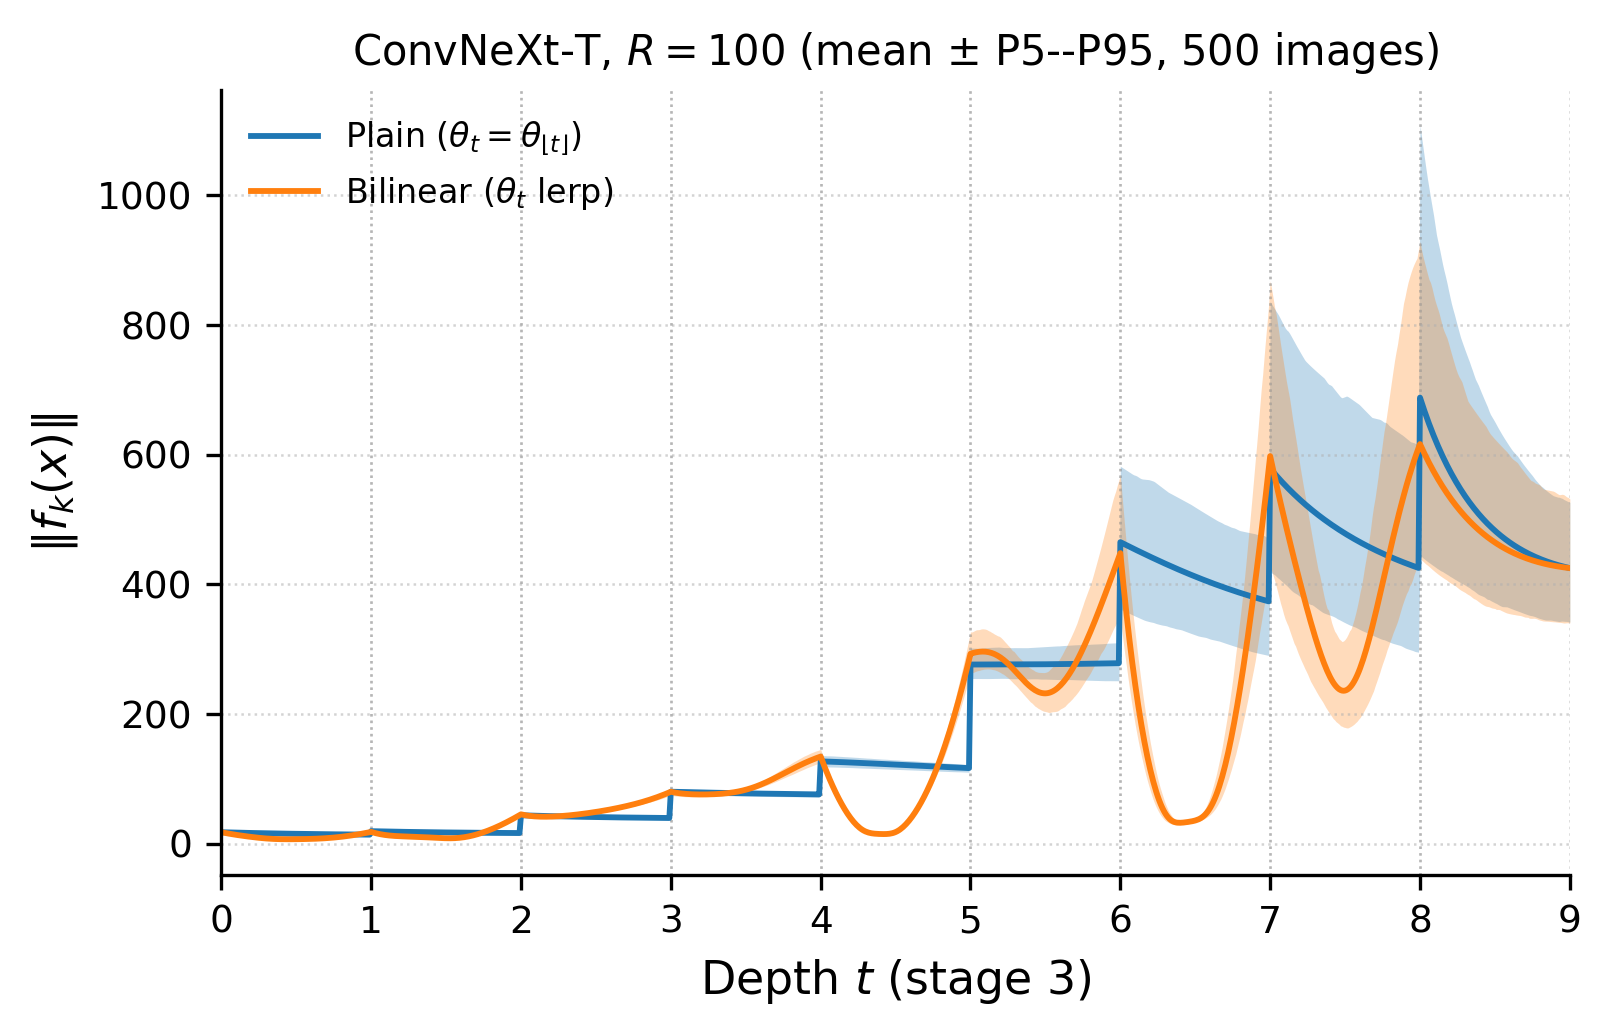
\includegraphics[width=\linewidth]{figures/bilinear_norm.png}
    \caption{ConvNeXt-T residual norm along stage~3 at $R{=}100$:
    plain vs.\ bilinear weight interpolation (mean and P5--P95 over 500 images).}
    \label{fig:bilinear-norm}
\end{figure}


\end{document}
